\chapter{Implementacja systemu}
\label{cha:implementacja}

Celem omawianego rozdziału jest przedstawienie implementacji proponowanego w Rozdziale \ref{cha:propozycja-systemu} systemu automatyki domowej. Niniejsza część została podzielona na dwie sekcje. W pierwszej sekcji zaprezentowana zostanie stworzona na potrzeby projektu sieć Thread. Kolejny fragment poświęcony jest warstwie aplikacji, technologiom wykorzystanym przy wdrażaniu komponentów oraz zasadzie działania systemu.

Projekt aplikacji systemu znajduje się w stworzonym przez autora pracy repozytorium \cite{project-repo}.

\section{Sieć Thread}

    \subsection{Założenia}
    \label{sec:thread-network-assumptions}
    
        Do stworzenia sieci Thread wykorzystano 5 urządzeń Nordic Semiconductor nRF52833 oraz Laptop Dell G3 15 z procesorem Intel Core i7 9. generacji, z systemem operacyjnym Microsoft Windows 11. Przed przystąpieniem do procesu implementacji sieci Thread, dokonano następujących założeń:
        \begin{itemize}
            \item Jedna platforma nRF52833 wraz z laptopem Dell zostaną wykorzystane do pełnienia roli Rutera brzegowego.
            \item Dwa urządzenia nRF52833 zostaną skonfigurowane do typu MTD oraz będą stanowiły urządzenia końcowe, MED oraz SED, które w warstwie aplikacji będą pełniły rolę profili HEATER oraz DIMMER.
            \item Dwa urządzenia nRF52833 zostaną skonfigurowane do typu FTD. Zostaną one wprowadzone do sieci, aby zapewnić nadmiarowość i pozwolić Liderowi Thread na dostosowanie topologii do aktualnych potrzeb i wymagań sieci.
        \end{itemize}

        Na Rysunku \ref{fig:thread-topology} przedstawiono przykładową topologię sieci Thread, złożoną z wyszczególnionych powyżej urządzeń.

        \begin{figure}[H]
            \centering
            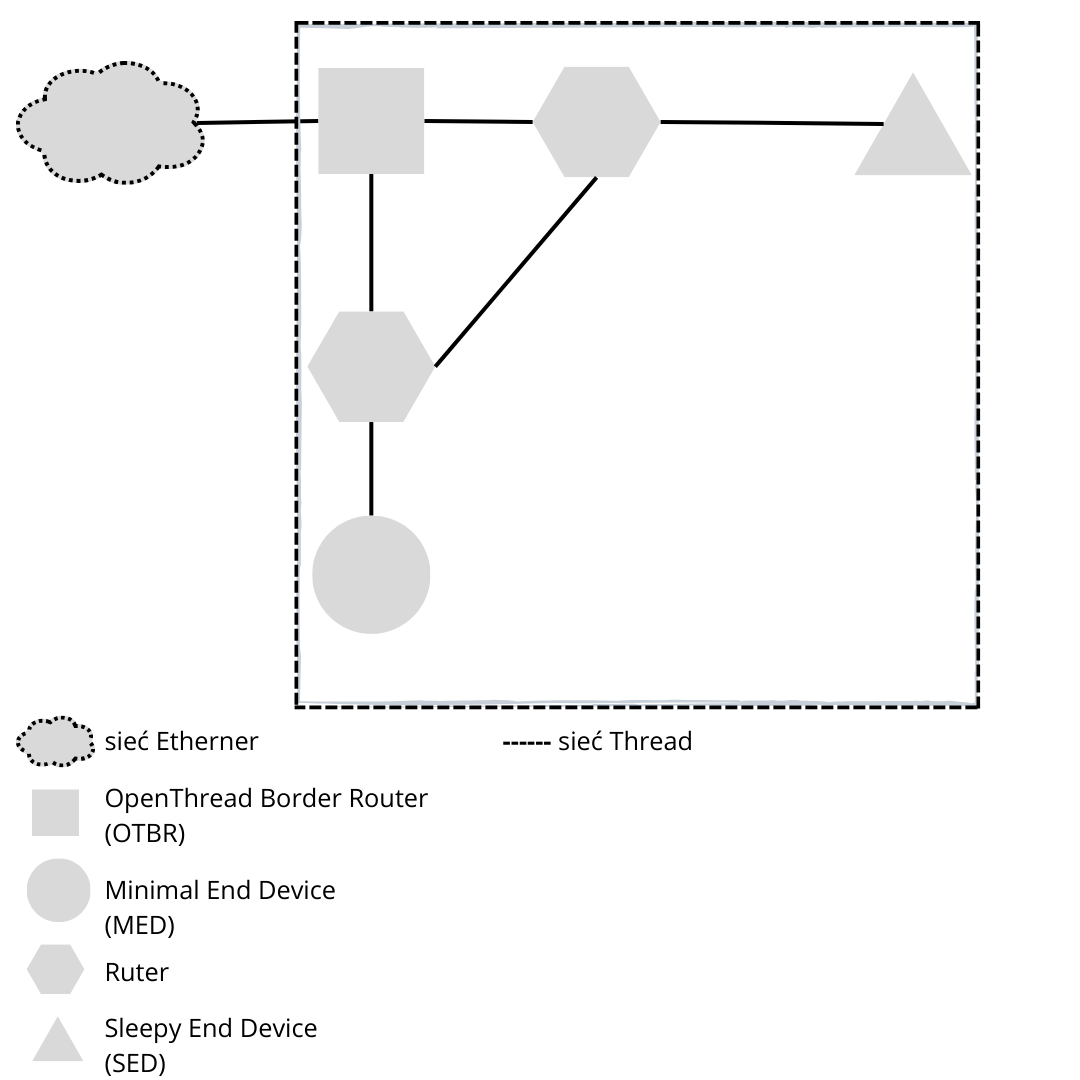
\includegraphics[width=0.8\linewidth]{graphics/thread-topology.png}
            \caption{Przykładowa topologia sieci Thread złożona z urządzeń wymienionych w założeniach w Sekcji \ref{sec:thread-network-assumptions}.}
            \label{fig:thread-topology}
        \end{figure}

    \subsection{Ruter Brzegowy}
    \label{subsec:otbr-implementation}

        W celu zapewnienia komunikacji przyszłej sieci Thread z zewnętrzną siecią Ethernet, w pierwszej kolejności przystąpiono do konfiguracji Rutera brzegowego, wykorzystując implementację OTBR. 
        
        Aplikacja OTBR jest dedykowana dla systemów operacyjnych Linux oraz do poprawnego działania wymaga nawiązania komunikacji zarówno z interfejsem sieci Thread, jak i z interfejsem sieci zewnętrznej. Z tego powodu, w początkowym kroku skonfigurowano platformę Linux jako maszynę wirtualną z dystrybucją Ubuntu tak, aby zapewnić komunikację sieciową oraz komunikację portów szeregowych między urządzeniem gościa (ang. \textit{Guest}) (maszyną wirtualną) a gospodarza (ang. \textit{Host}) (Laptop Dell). Kolejno skonfigurowano środowisko deweloperskie, instalując narzędzia takie jak system kontroli wersji Git oraz IDE (ang. \textit{Integrated Development Environment}). 

        Po weryfikacji poprawności działania maszyny wirtualnej kontynuowano proces konfiguracji OTBR, wykorzystując instrukcję zamieszczoną na oficjalnej stronie projektu OpenThread \cite{otbr-docker}. Zaprogramowano jedno z urządzeń nRF52833 aplikacją RCP (ang. \textit{Radio Co-Processor}), używając dostarczonej przez OpenThread implementacji \cite{otbr-rcp-app}. Ostatecznie zainstalowano oprogramowanie Docker oraz pobrano dystrybuowany przez OpenThread kontener.

        Tak przygotowane środowisko Linux oraz zaprogramowane urządzenie nRF52833 są gotowe do uruchomienia w pełni funkcjonalnej aplikacji Rutera Brzegowego.

    \subsection{Urządzenia MTD oraz FTD}
    \label{subsubsec:mtd-ftd-devices-implementation}

    Aplikację dla 4 pozostałych urządzeń nRF52833 stworzono w języku C z wykorzystaniem nRF Connect SDK oraz środowiska programistycznego nRF Connect IDE. W plikach konfiguracyjnych projektów skonfigurowano odpowiednio stos protokołu i niezbędne funkcjonalności Thread, system logowanie, GPIO (ang. \textit{general-purpose input/output}). Kolejno wybrano tryb MTD dla 2 urządzeń, natomiast dla pozostałych FTD. 

    Co więcej, w urządzeniach MTD uwzględniono możliwość przejścia w tryb energooszczędny, poprzez naciśnięci przycisku Button 3, w wyniku czego ED zmienia pełniącą rolę z MED na SED oraz obniża zużycie energii w wyniku ograniczenia zużycia pamięci RAM.

    Na potrzeby procesu rozwoju oprogramowania, wzbogacono wszystkie 4 platformy, o sygnalizację stanu urządzenia Thread przy pomocy LED (ang. \textit{light-emitting diode}). Dioda LED1 świeci się, gdy urządzenie Thread jest włączone do sieci.
    
\section{Warstwa Aplikacji}

    Do wymiany informacji podczas komunikacji klient-serwer między urządzeniami końcowymi w sieci Thread a System Controllerem, wykorzystano protokół warstwy aplikacji Constrained Application. CoAP jest protokołem opartym o REST API (ang. \textit{Representational State Transfer Application Programming Interface}), który nawiązuje połączenie z wykorzystaniem wspieranego przez stos Thread protokołu UDP.

    \subsection{Implementacja komponentów systemy}

        Obecna sekcja ma za zadanie przybliżyć szczegóły implementacji poszczególnych komponentów wymienionych w Rozdziale \ref{cha:propozycja-systemu}.

        \subsubsection{Baza danych}
            Przez wzgląd na mały rozmiar, pełne wsparcie funkcjonalności SQL (ang. \textit{Structured Query Language}) oraz możliwość przechowywania bazy danych w pojedynczym pliku, jako silnik wykorzystywanej w projekcie systemu Bazy Danych wybrano SQLite. \cite{sqlite}.

            Stworzony na potrzeby systemu zestaw tabel Bazy Danych przedstawiono na Rysunku \ref{fig:db-diagram}.

            \begin{figure}[H]
                \centering
                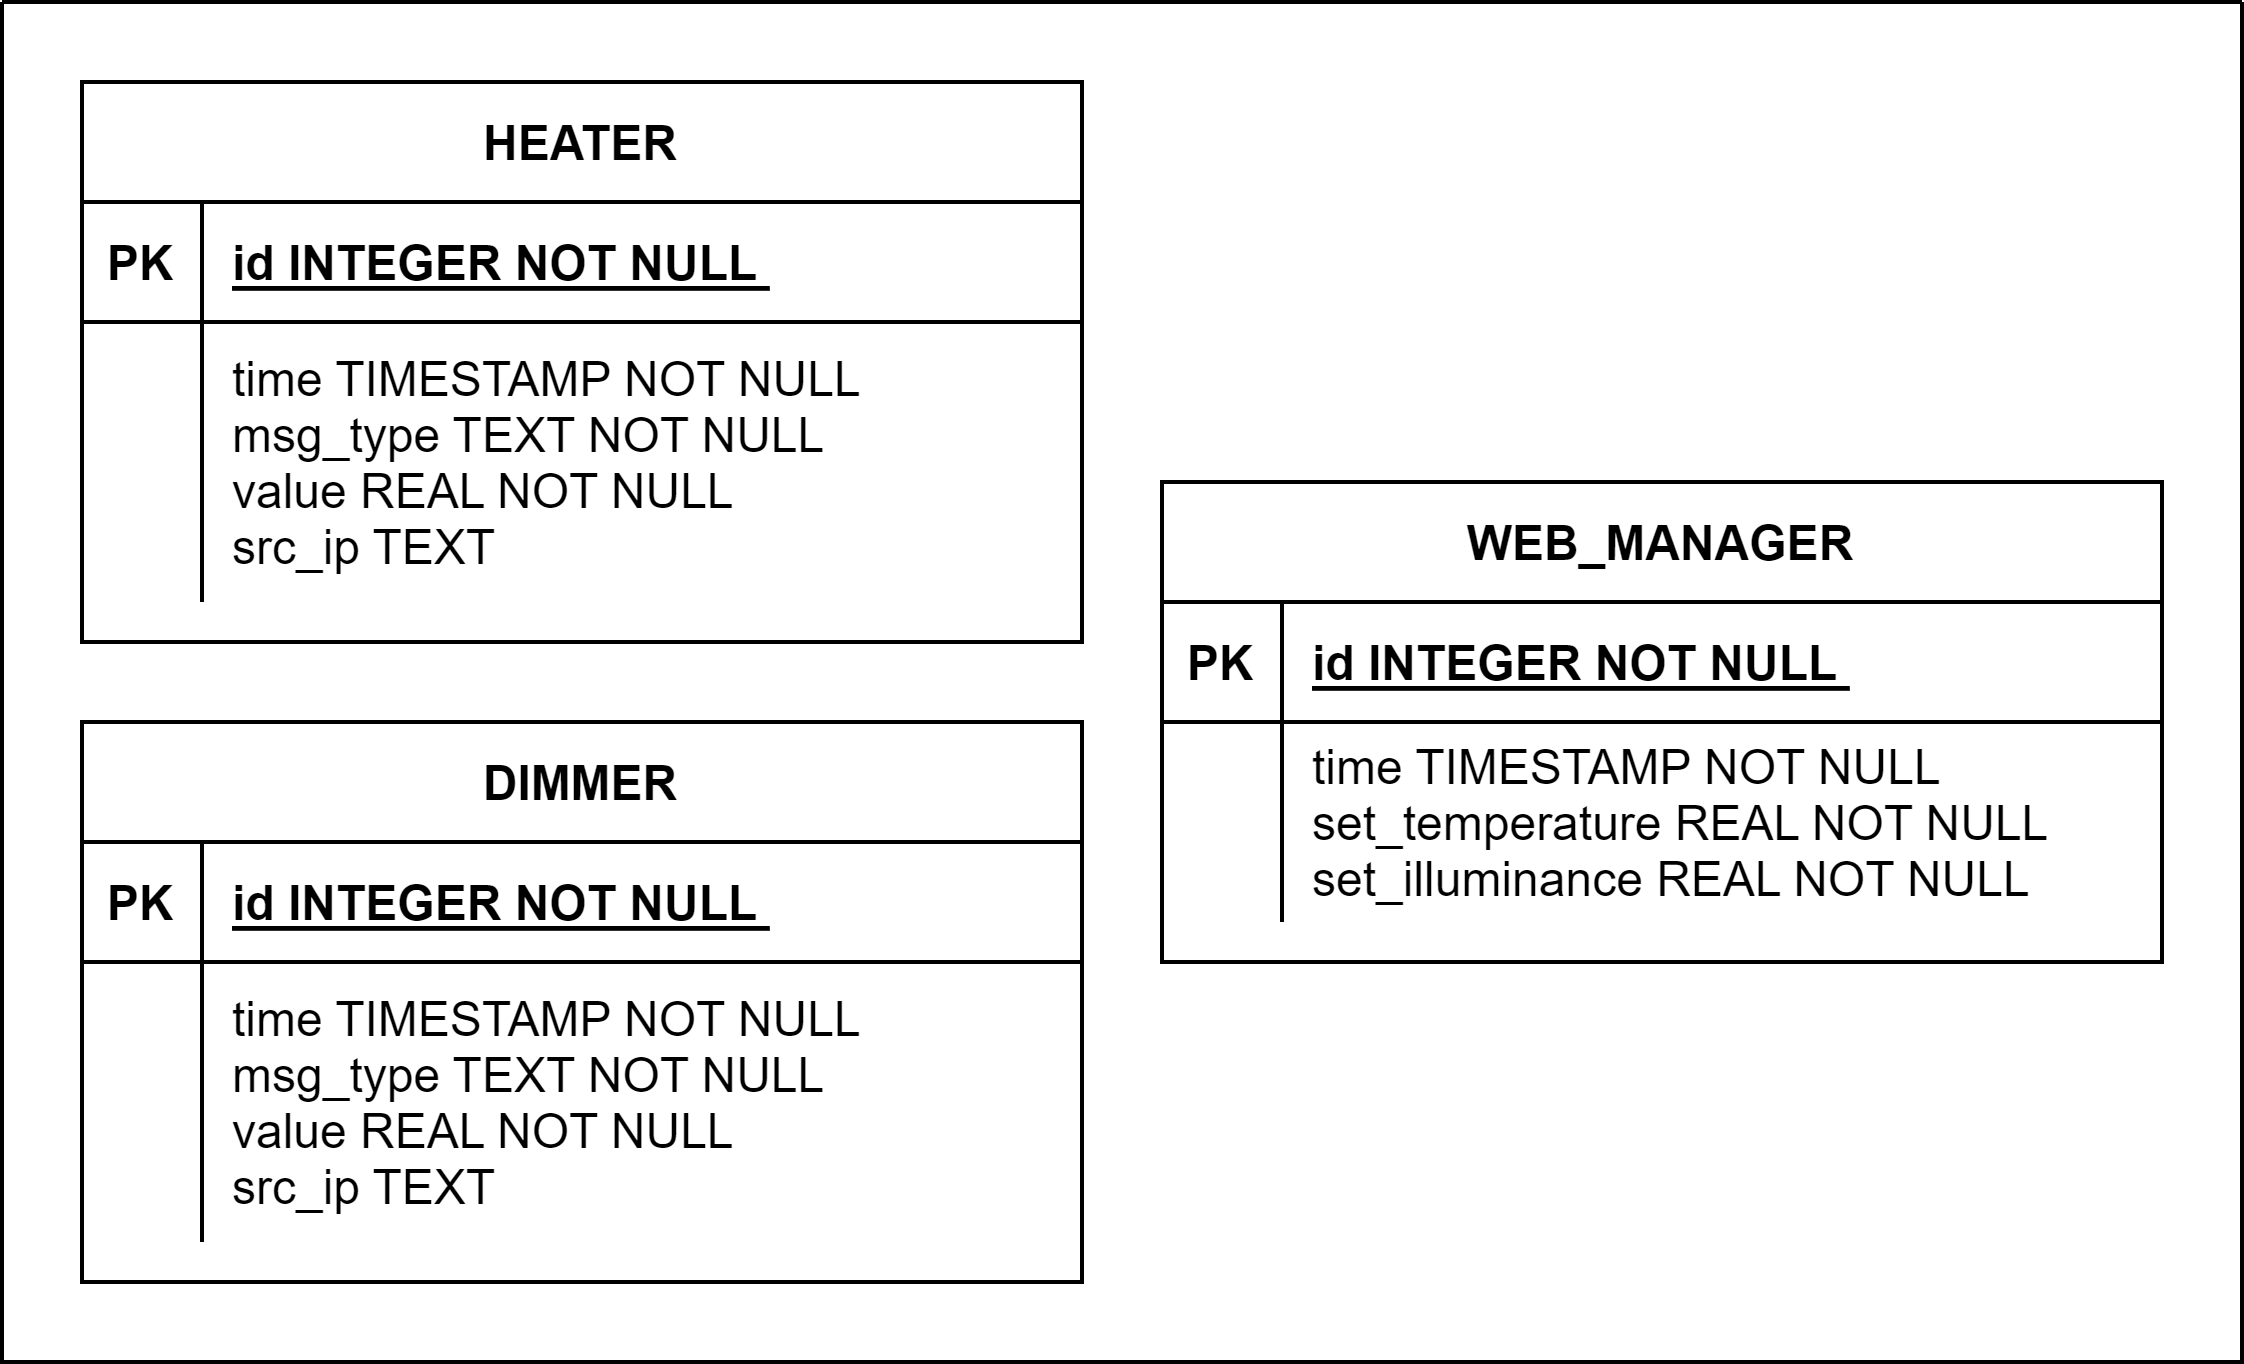
\includegraphics[width=0.8\linewidth]{graphics/db_diagram.png}
                \caption{Schemat tabel Bazy Danych systemu.}
                \label{fig:db-diagram}
            \end{figure}

            Tabela WEB\_MANAGER ma za zadanie przechowywać wpisy dotyczące ustawionych przez użytkownika parametrów. Tablica HEATER oraz tablica DIMMER zawierają informację o kolejnych przetworzonych przez System Controller żądaniach CoAP.
    
        \subsubsection{System Controller}
    
            System Controller został wdrożony jako aplikacja w języku Python, przeznaczona dla urządzeń z systemem operacyjnym Linux.
            System Controller odbiera żądania oraz wysyła odpowiedzi CoAP z wykorzystaniem dostarczonego przez bibliotekę aiocoap API \cite{aiocoap}. URI (ang. \textit{Uniform Resource Identifier}) zdefiniowanych zasobów serwera, obsługiwany typ zapytań oraz ich funkcje, zestawiono w Tabeli \ref{tab:resurces}.
            
            Zarządzanie Bazą Danych SQLite odbywa się z użyciem wbudowanych w język Python bibliotek \textit{sqlite3} oraz \textit{aiosqlite}.

            \begin{table}[H]
                \centering
                \caption{Zasoby serwera CoAP.}
                \begin{tabular}{|l|l|l|}
                     \hline
                     \rowcolor{gray!20}
                     \multicolumn{1}{|c|}{Zasób} & \multicolumn{1}{c|}{Typ zapytań} & \multicolumn{1}{c|}{Funkcja} \\
                     \hline
                     temperature & GET, PUT & Przechowuje wartość aktualnej temperatury środowiska.\\
                     \hline
                     illuminance & GET, PUT & Przechowuje wartość aktualnego natężenia oświetlenia środowiska.\\
                     \hline
                     heater\_regulation & GET & Zwraca wartość parametru regulacji dla układu HEATER.\\
                     \hline
                     dimmer\_regulation & GET & Zwraca wartość parametru regulacji dla układu DIMMER.\\
                     \hline
                \end{tabular}
                \label{tab:resurces}
            \end{table}
    
        \subsubsection{HEATER oraz DIMMER}

            Platformy nRF52833 pracujące jako MTD, w których skonfigurowano stos Thread, jak opisano w Podsekcji \ref{subsubsec:mtd-ftd-devices-implementation}, wzbogacono o warstwę aplikacji. Urządzenia Końcowe symulują zachowanie zdefiniowanych w Sekcji \ref{sec:system-clients} profili HEATER oraz DIMMER. Wysyłanie zapytań oraz odbieranie odpowiedzi CoAP zaimplementowano z wykorzystaniem API dostarczonego przez nRF Connect SDK, oraz OpenThread.

            W urządzeniach HEATER oraz DIMMER skonfigurowano przycisk Button 3, którego naciśnięcie inicjalizuje stronę klienta CoAP oraz pobiera z sieci prefiks NAT64, niezbędny do nawiązania połączenia z serwerem o skonfigurowanym IPv4.
        
        \subsubsection{Web GUI}

            Interfejs użytkownika Web GUI stanowi aplikacja w języku Python, którą stworzono z użyciem następujących technologii webowych:
            \begin{itemize}
                \item mikro-frameworku Flask \cite{flask},
                \item CSS (ang. \textit{Cascading Style Sheets}),
                \item HTML (ang. \textit{HyperText Markup Language}).
            \end{itemize}
            Aplikacja komunikuje się bezpośrednio z bazą danych, wykorzystując bibliotekę sqlite3.

            \begin{figure}[H]
                \centering
                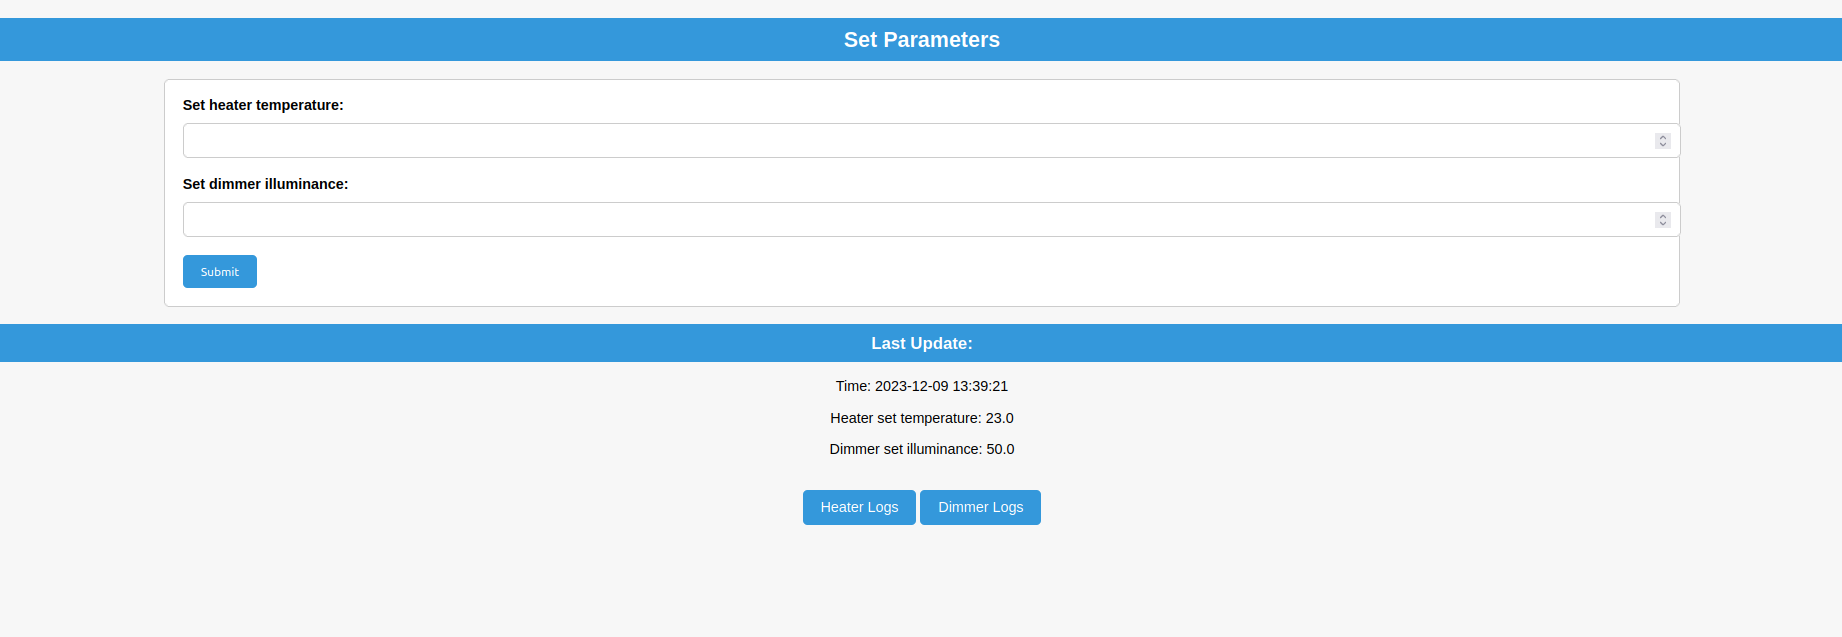
\includegraphics[width=0.8\linewidth]{graphics/screenshots/web-gui-set-parameters.png}
                \caption{Zrzut ekranu przedstawiający panel Web GUI przeznaczony do ustalania parametrów systemu.}
                \label{fig:web-gui-set-parameters}
            \end{figure}

            \begin{figure}[H]
                \centering
                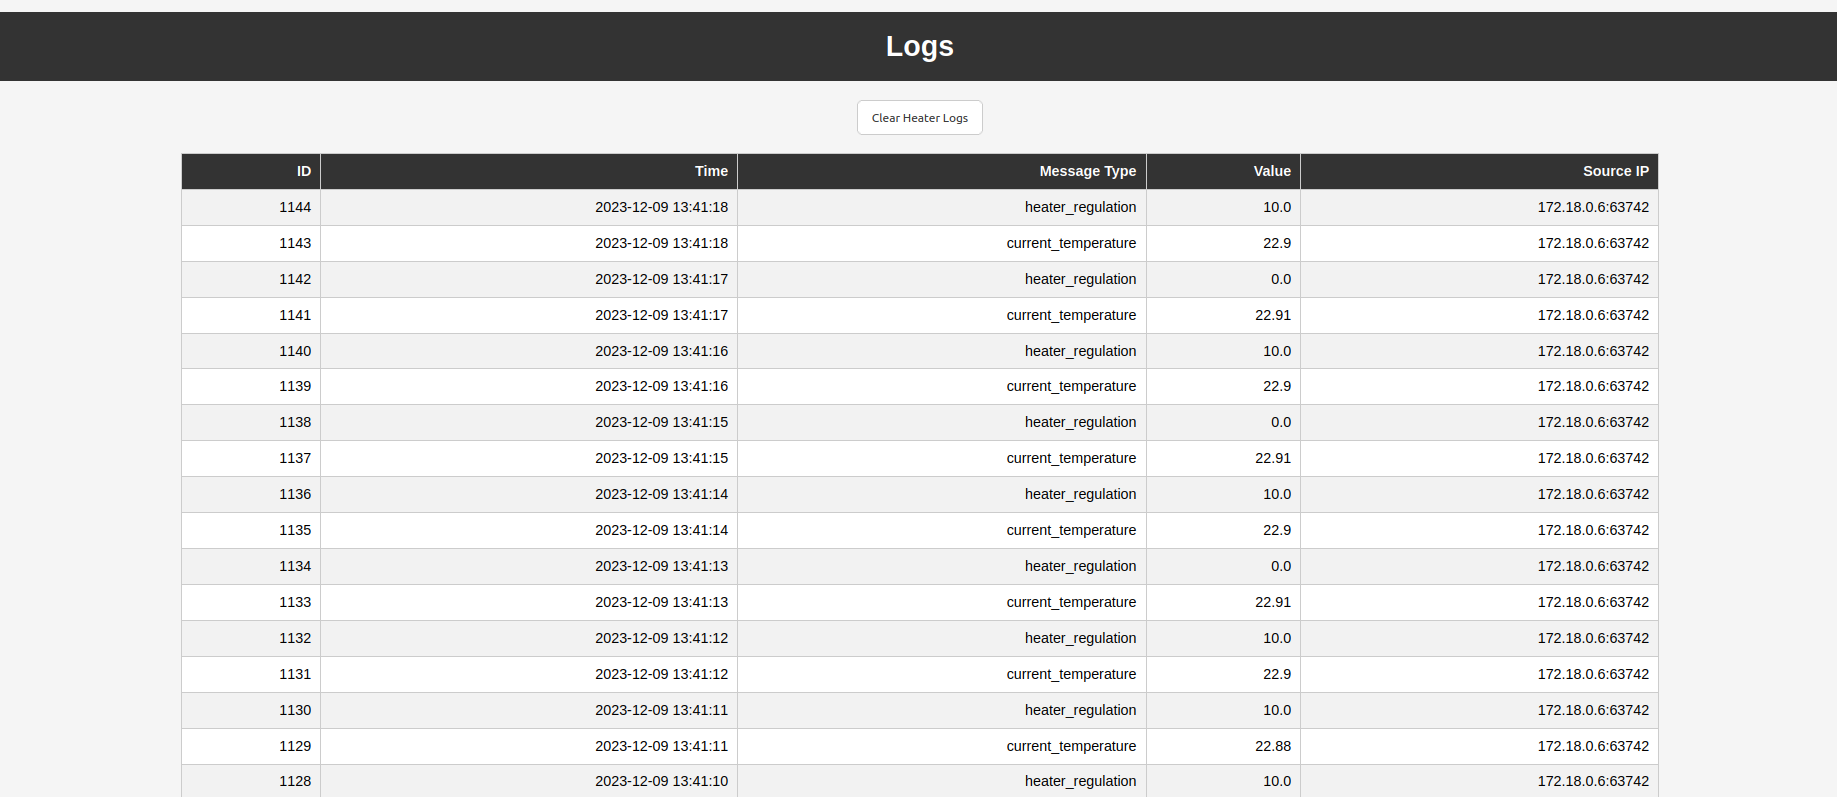
\includegraphics[width=0.8\linewidth]{graphics/screenshots/web-gui-logs.png}
                \caption{Zrzut ekranu przedstawiający panel Web GUI przeznaczony do obserwacji logów systemu.}
                \label{fig:web-gui-logs}
            \end{figure}

    \subsection{Symulacja}
    W wyniku założenia o symulacyjnym charakterze prototypowego systemu tj. braku uwzględnienia rzeczywistych czujników oraz układów regulacyjnych zaimplementowano ekosystem, który stanowi pewne przybliżenie środowiska, w którym mógłby operować system. 

    W układach HEATER oraz DIMMER zasymulowano zmiany temperatury, oraz natężenia oświetlenia z wykorzystaniem licznika systemowego. Wraz z przerwaniem licznika, które dla HEATER następuje co 100ms, natomiast dla DIMMER co 200ms, aktualna temperatura oraz aktualne natężenie oświetlenia zastępowane są nową temperaturą, oraz nowym natężeniem oświetlenia. 

    Temperatura środowiska w układzie HEATER opisana jest następującym wzorem:
        \[nowa\_temperatura = aktualna\_temperatura + a\cdot parametr\_regulacji + b\]
    Gdzie:
    \begin{itemize}
        \item \textit{a = 0,00025},
        \item \textit{b = -5a}. 
    \end{itemize}

    Natomiast zmiany natężenia środowiska w układzie DIMMER opisuje funkcja:
    \[nowe\_no= aktualne\_no + a\cdot parametr\_regulacji\]
    Gdzie:
    \begin{itemize}
        \item \textit{nowe\_no} - nowe natężenie oświetlenia,
        \item \textit{aktualne\_no} - aktualne natężenie oświetlenia,
        \item \textit{a = 0,00025}
    \end{itemize}

    Wprowadzony parametr b we wzorze na chwilową temperaturę ekosystemu w układzie HEATER pozwala na zasymulowanie powolnego spadku temperatury. Środowisko wdrożone w Układzie DIMMER można przyjąć za izolowane, ponieważ nie uwzględnia żadnych zewnętrznych źródeł światła.
    Parametry a oraz b dla obydwu układów, zostały wyznaczone empirycznie, aby zagwarantować możliwość zaobserwowania zmian wynikających z poprawnego działania systemu.
    
    \subsection{Zasada działania}
    \label{subsec:system-behaviour}

    Celem niniejszej podsekcji jest opisanie zasady działania wdrożonego systemu automatyki domowej, poprzez przegląd logiki aplikacji oraz przepływu informacji między komponentami.
    
    Zachowanie systemu można podzielić na 3 fazy:
    \begin{itemize}
        \item Fazę ustalania parametrów systemu - użytkownik nadaje systemowi stan, do którego mają dążyć układy regulacyjne.
        \item Fazę pomiarów - układ pomiarowy przesyła aktualny stan parametru System Controllerowi.
        \item Fazę regulacji - układ regulacji odpytuje System Controller o nową wartość parametru regulacji w celu utrzymania parametrów środowiska dążących do zadanego przez użytkownika stanu.
    \end{itemize}

    Ustalanie parametrów systemu odbywa się asynchronicznie przez użytkownika, natomiast regulacja oraz pomiar wykonywane są periodycznie z okresem 1s.

        \subsubsection{Ustalanie parametrów systemu}

            Na Rysunku \ref{fig:seq-user-webgui-db} zilustrowano przepływ wiadomości między komponentami systemu w fazie ustalania parametrów systemu.

            \begin{figure}[H]
                \centering
                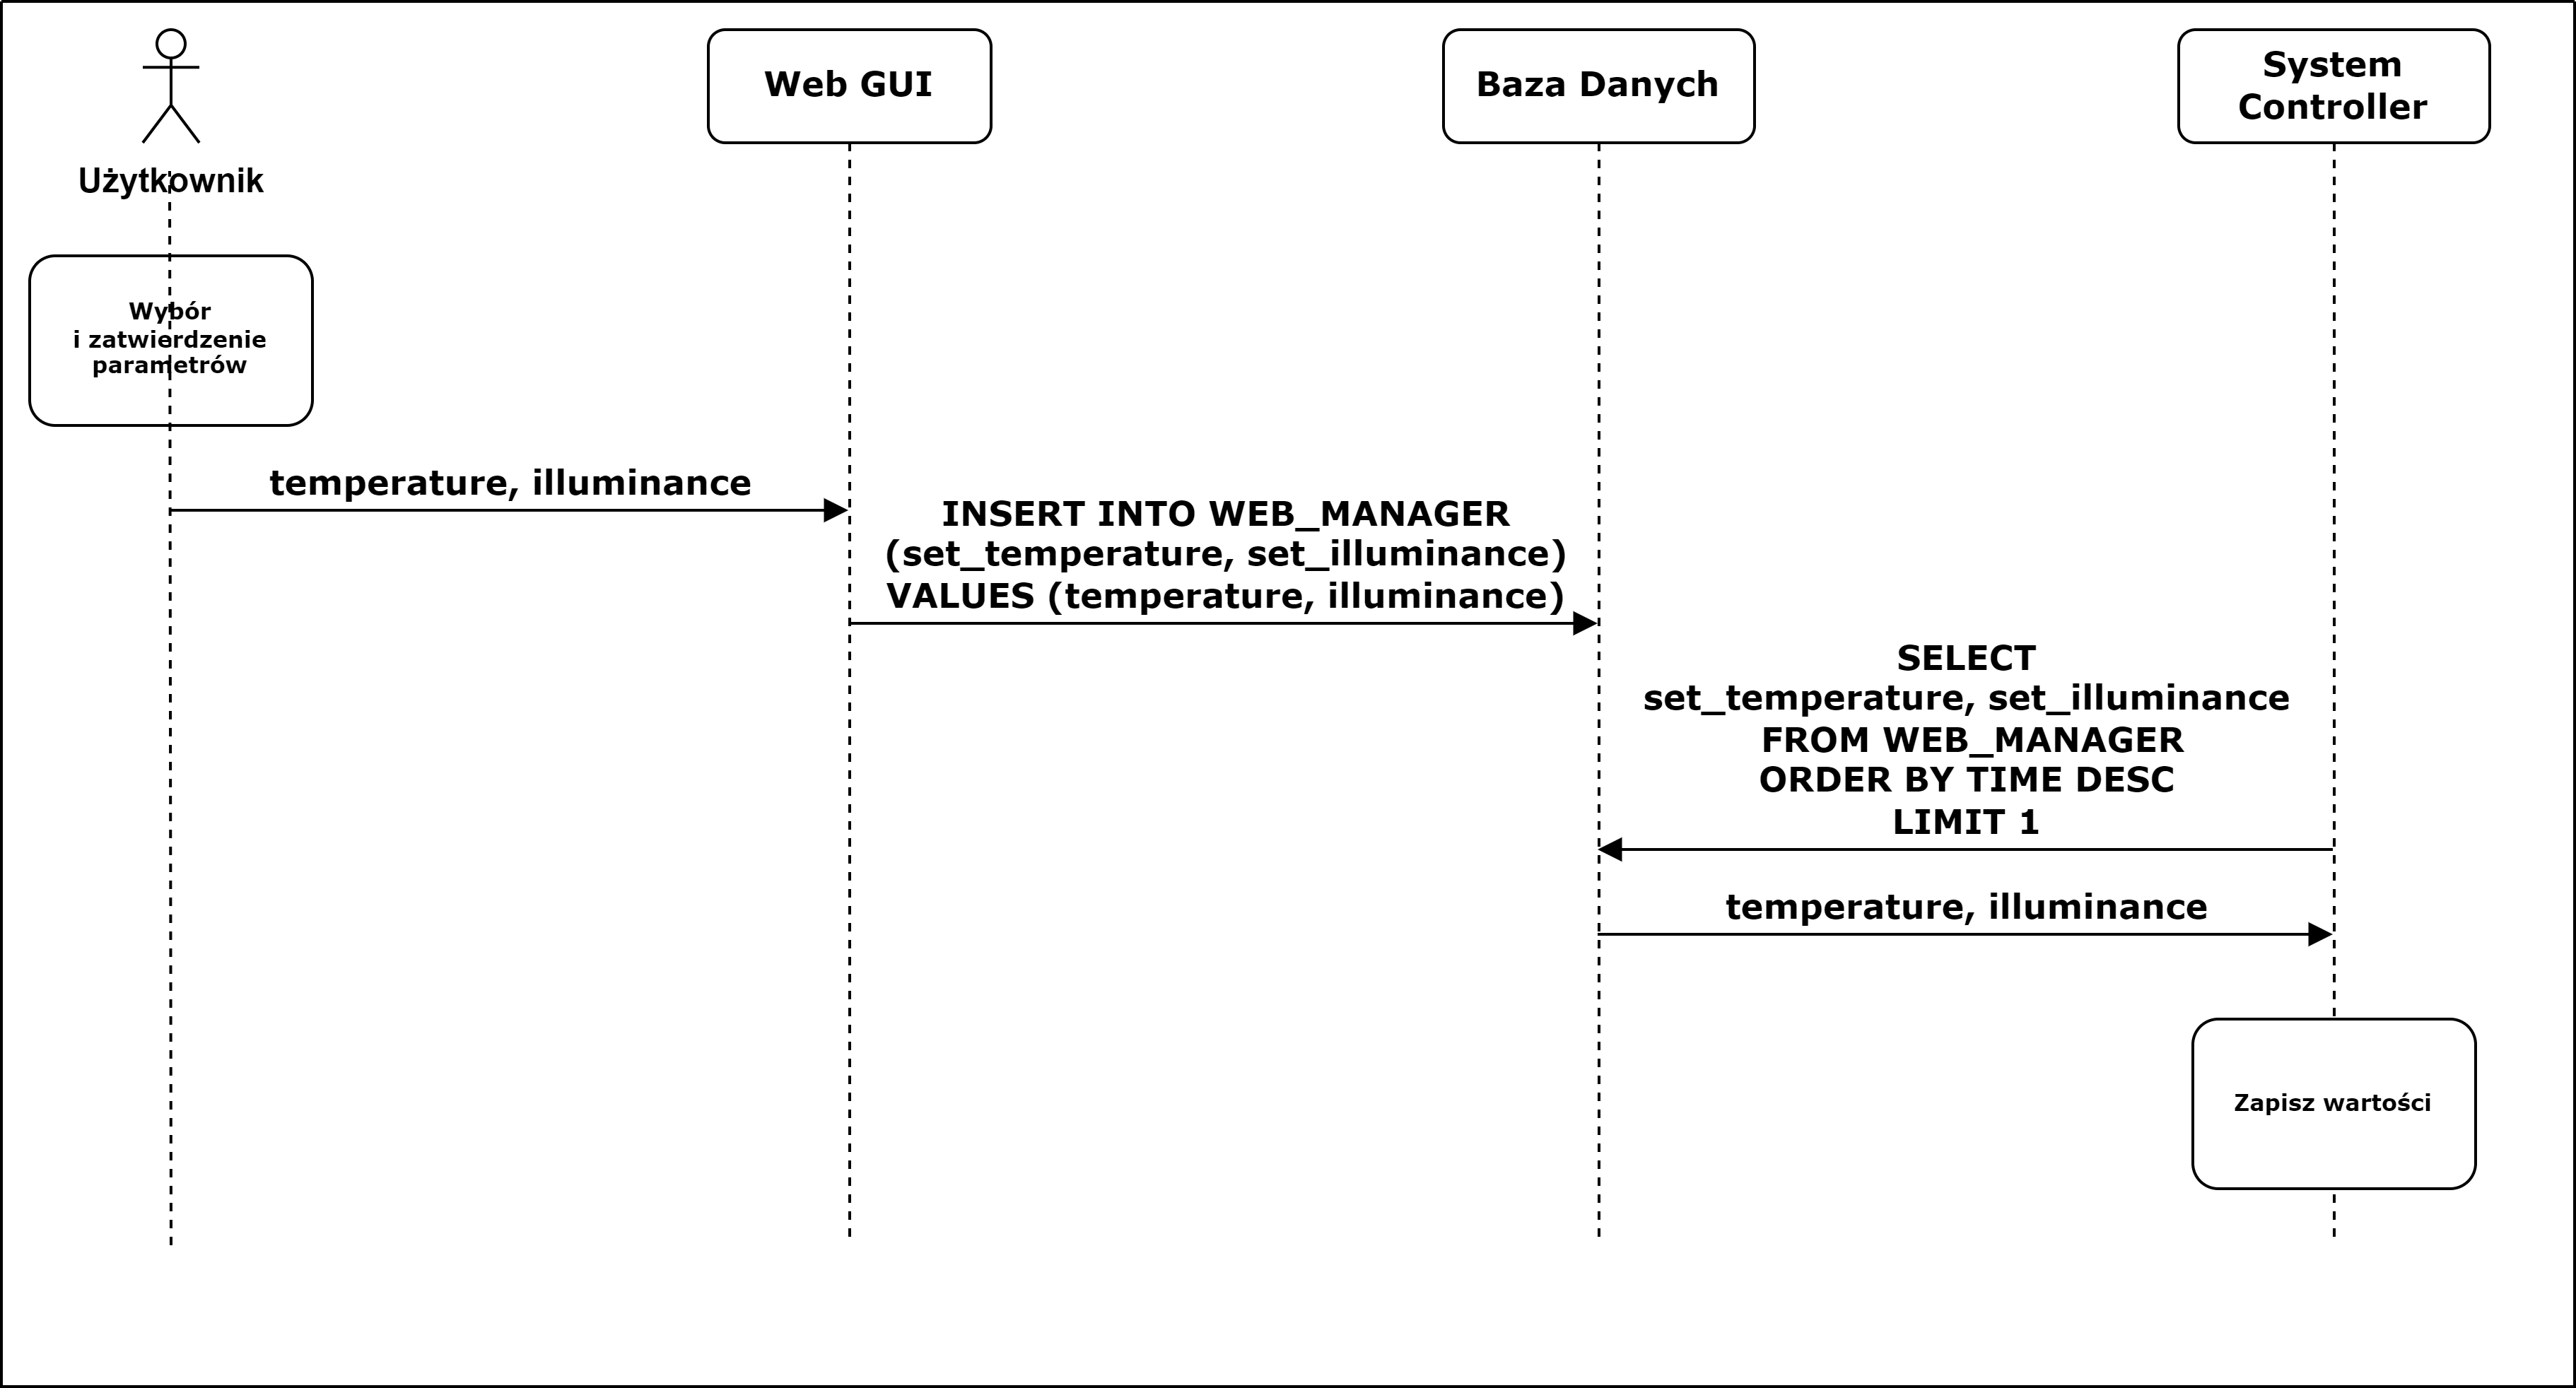
\includegraphics[width=0.8\linewidth]{graphics/sequence-diagrams/user-webgui-db-diagram.png}
                \caption{Diagram sekwencji ustawiania parametrów systemu.}
                \label{fig:seq-user-webgui-db}
            \end{figure}

            Kolejnymi krokami procedury są:
            \begin{enumerate}
                \item Użytkownik korzystający z panelu Web GUI, służącego do ustawiania parametrów systemu, zobrazowanym na Rysunku \ref{fig:web-gui-set-parameters}, podaje i zatwierdza wartości.
                \item Wprowadzone wartości \textit{temperature} oraz \textit{illuminance} wstawiane są do tabeli WEB\_MANAGER Bazy Danych.
                \item System Controller cyklicznie odpytuje Bazę Danych o ostatnio zaktualizowane wartości temperatury i natężenia oświetlenia.
                \item Po uzyskaniu wartości \textit{temperature} oraz \textit{illuminance} System Controller zapisuje je w swoim programie.
            \end{enumerate}

        \subsubsection{Pomiar}

            Na Rysunku \ref{fig:seq-heater-measure} zilustrowano przepływ wiadomości między komponentami systemu w fazie pomiaru temperatury.

            \begin{figure}[H]
                \centering
                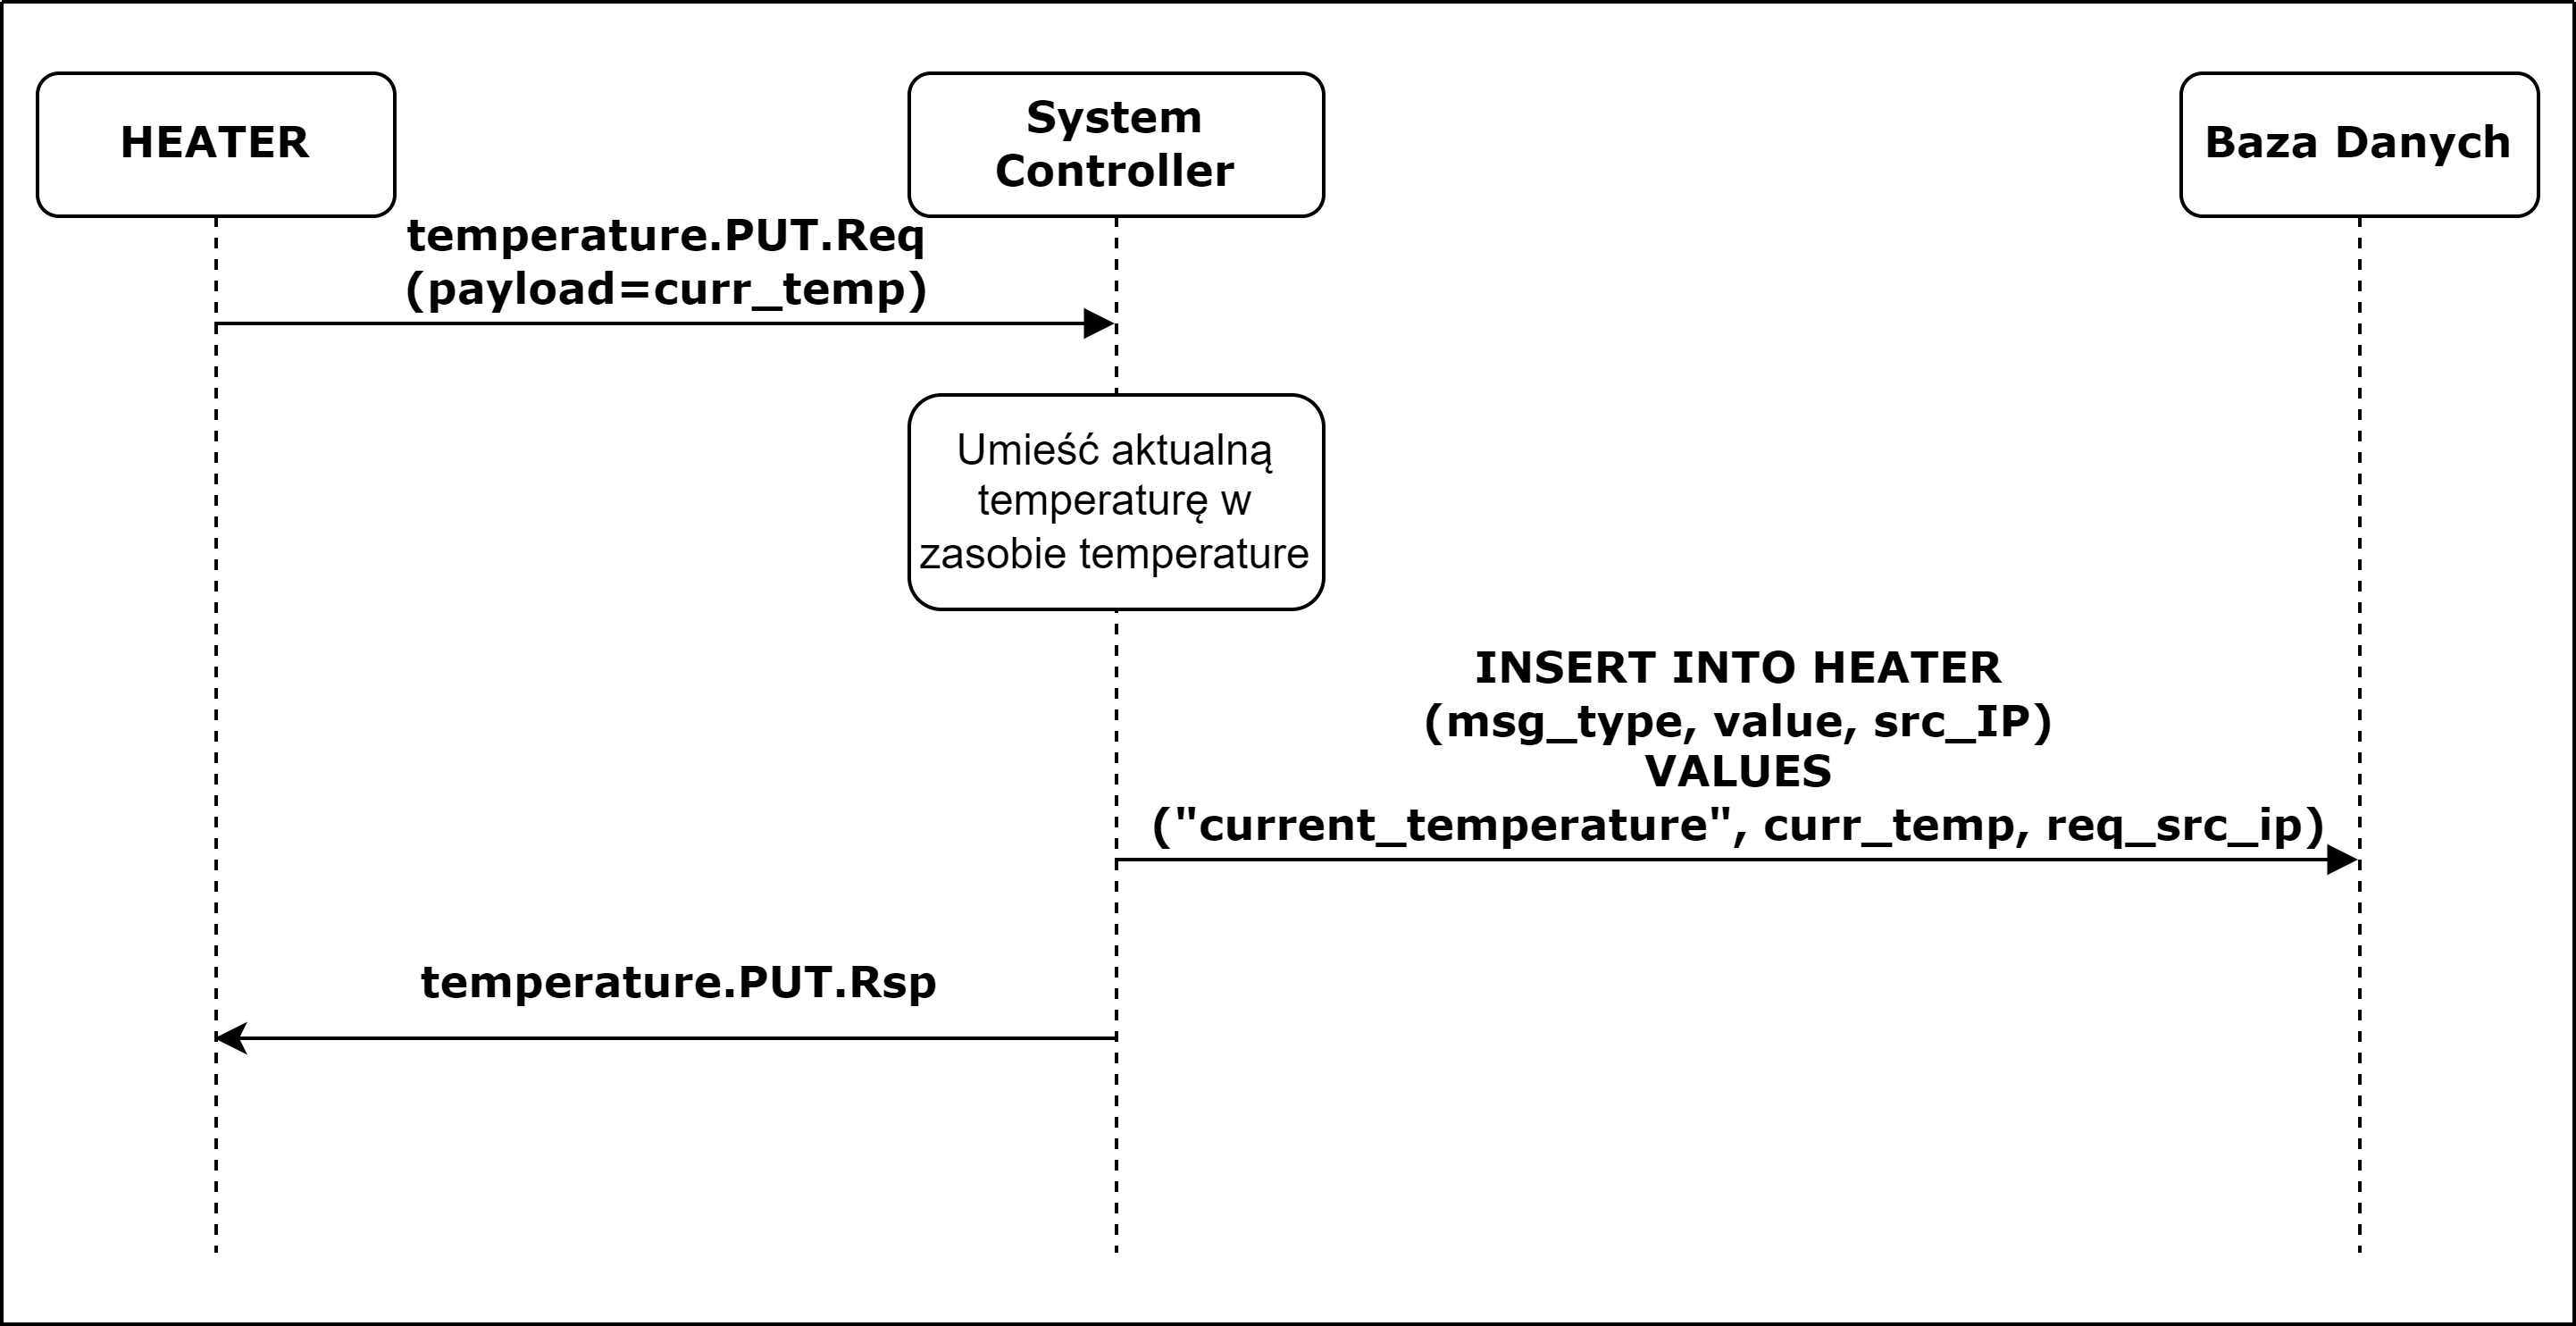
\includegraphics[width=0.8\linewidth]{graphics/sequence-diagrams/heater-measure-seq.png}
                \caption{Diagram sekwencji pomiaru temperatury.}
                \label{fig:seq-heater-measure}
            \end{figure}

            Kolejnymi krokami pomiaru temperatury w fazie pomiaru są:
            \begin{enumerate}
                \item Urządzenie HEATER wysyła zapytanie do System Controllera o umieszczenie aktualnej temperatury \textit{curr\_temp} w zasobie \textit{temperature}.
                \item System Controller umieszcza otrzymaną wartość \textit{curr\_temp} w zasobach serwera.
                \item System Controller loguje informację o przetworzonym zapytaniu, umieszczając otrzymaną wartość temperatury w tabeli HEATER Bazy Danych.
                \item System Controller w ramach potwierdzenia otrzymania zapytania odpowiada układowi HEATER.
            \end{enumerate}

            Na Rysunku \ref{fig:seq-dimmer-measure} zilustrowano przepływ wiadomości między komponentami systemu w fazie pomiaru natężenia oświetlenia.

            \begin{figure}[H]
                \centering
                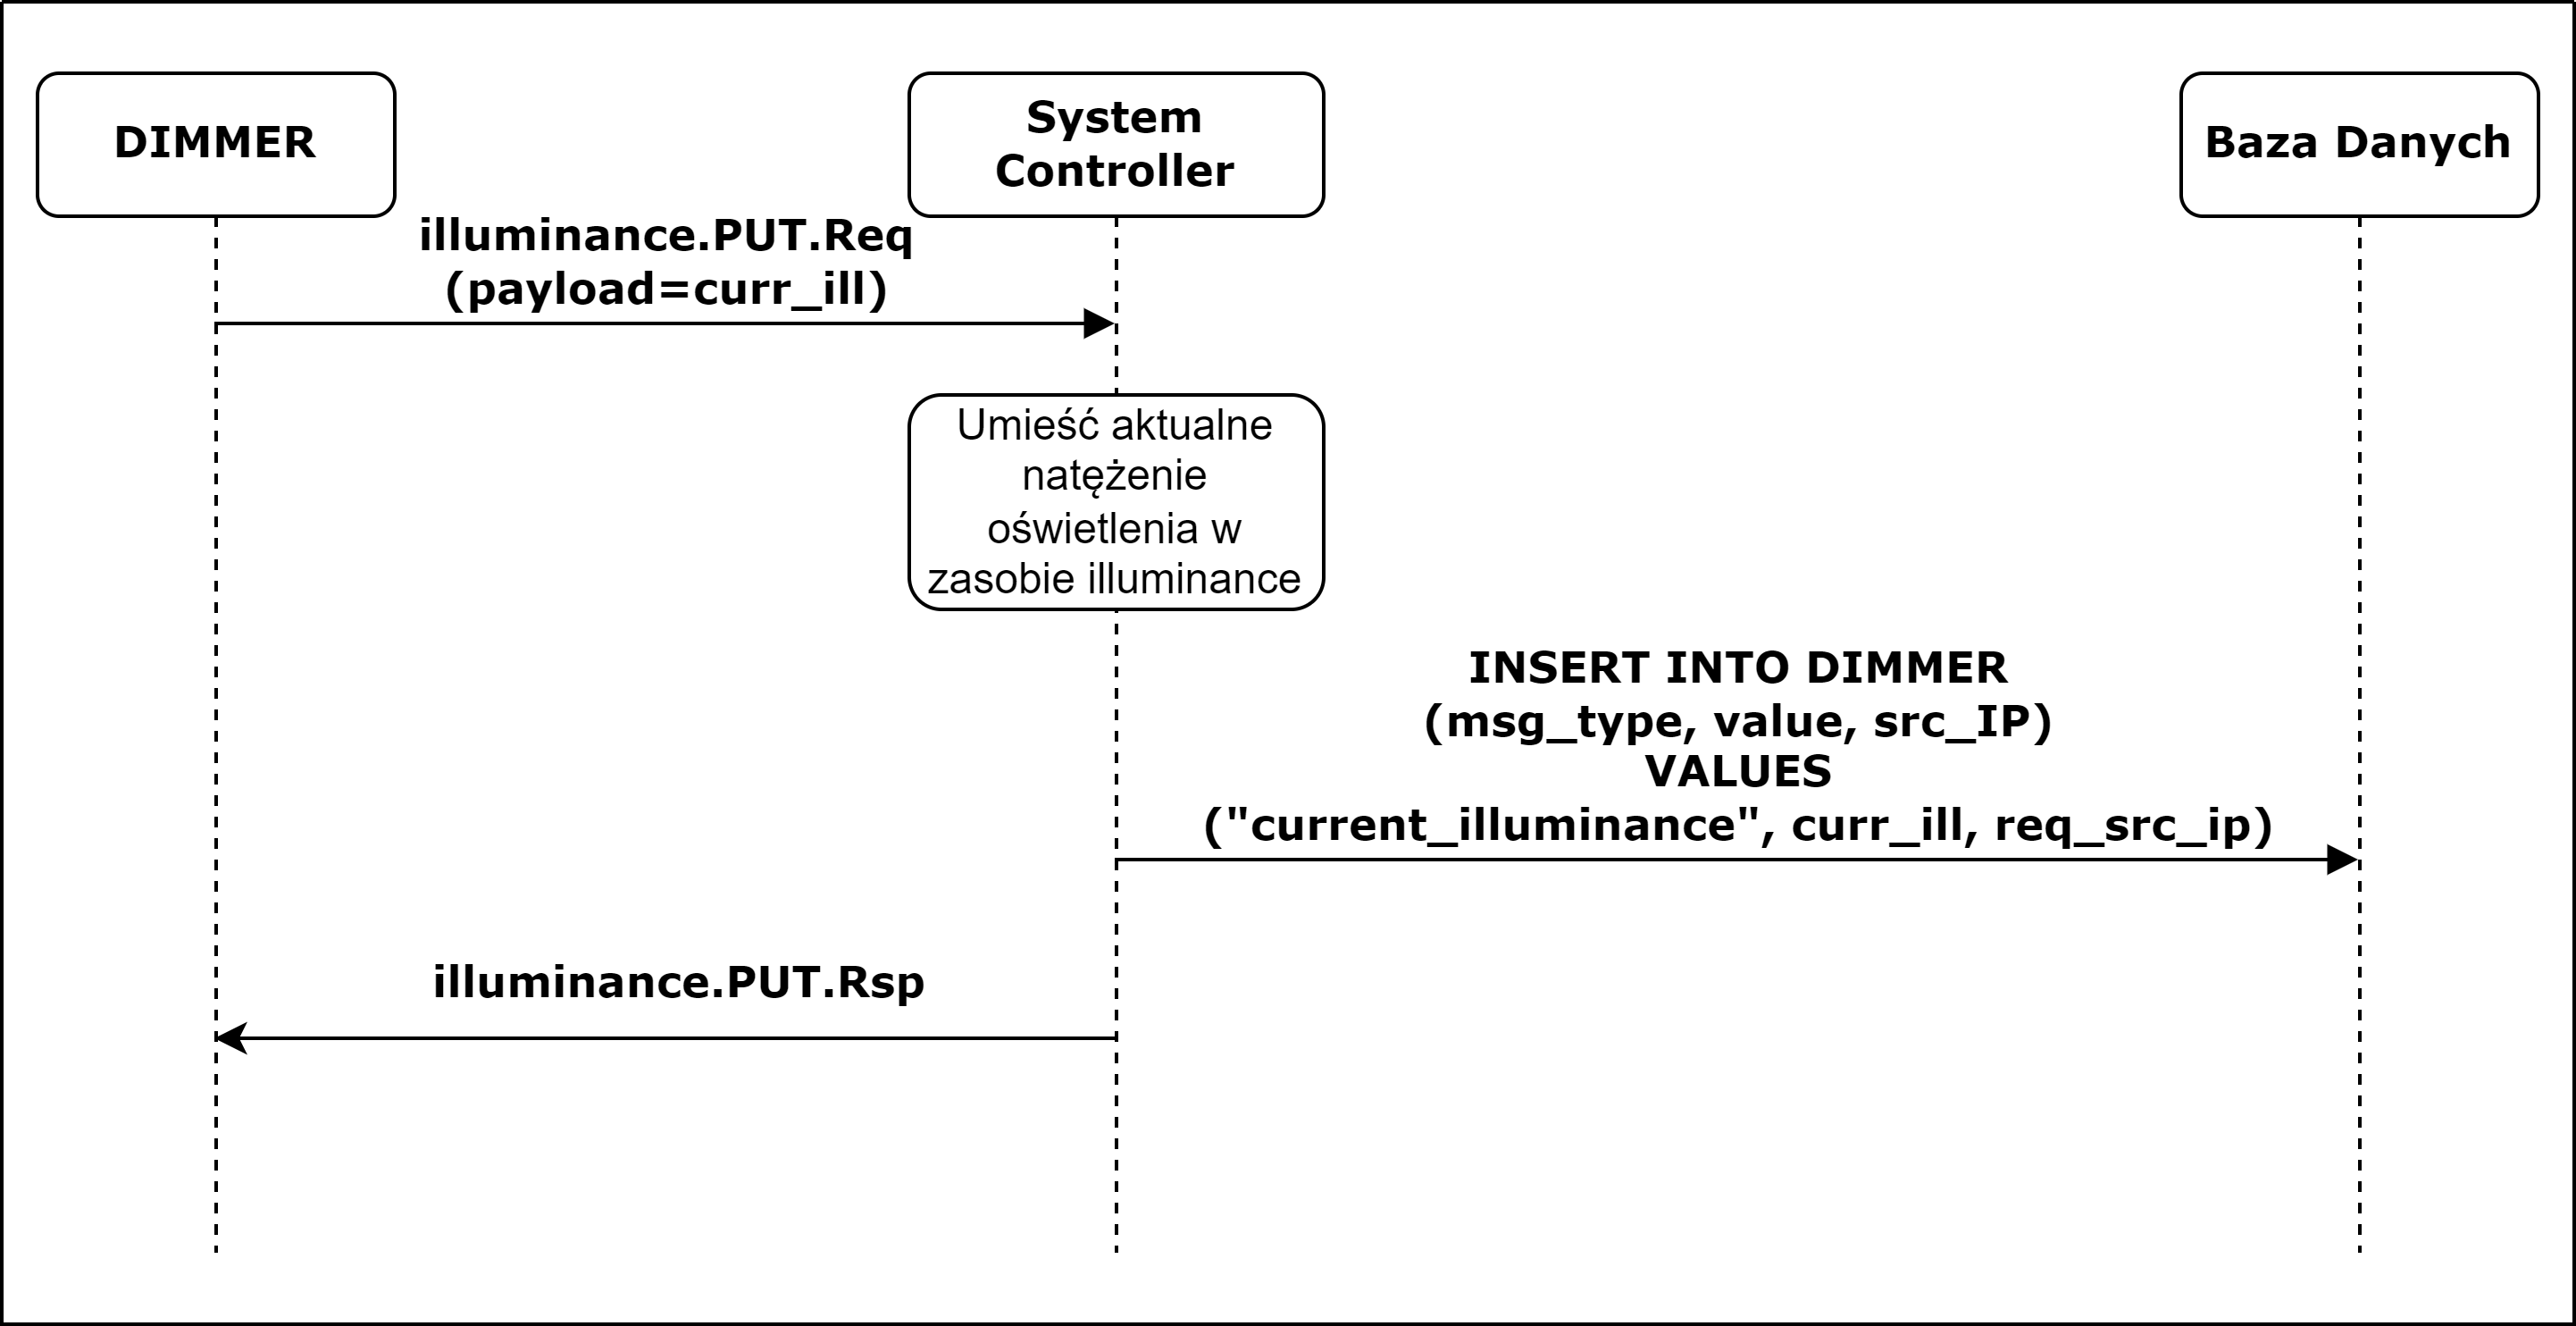
\includegraphics[width=0.8\linewidth]{graphics/sequence-diagrams/dimmer-measure-seq.png}
                \caption{Diagram sekwencji pomiaru natężenia oświetlenia.}
                \label{fig:seq-dimmer-measure}
            \end{figure}

            Kolejnymi krokami pomiaru natężenia oświetlenia w fazie pomiaru są:
            \begin{enumerate}
                \item Urządzenie DIMMER wysyła zapytanie do System Controllera o umieszczenie aktualnego natężenia oświetlenia \textit{curr\_ill} w zasobie \textit{illuminance}.
                \item System Controller umieszcza otrzymaną wartość natężenia oświetlenia \textit{curr\_ill} w zasobach serwera.
                \item System Controller loguje informację o przetworzonym zapytaniu, umieszczając otrzymaną wartość natężenia oświetlenia w tabeli DIMMER Bazy Danych.
                \item System Controller w ramach potwierdzenia otrzymania zapytania odpowiada układowy HEATER.
            \end{enumerate}


        \subsubsection{Regulacja}

            Na Rysunku \ref{fig:seq-heater-regulate} zilustrowano przepływ wiadomości między komponentami systemu w fazie regulacji temperatury.

            \begin{figure}[H]
                \centering
                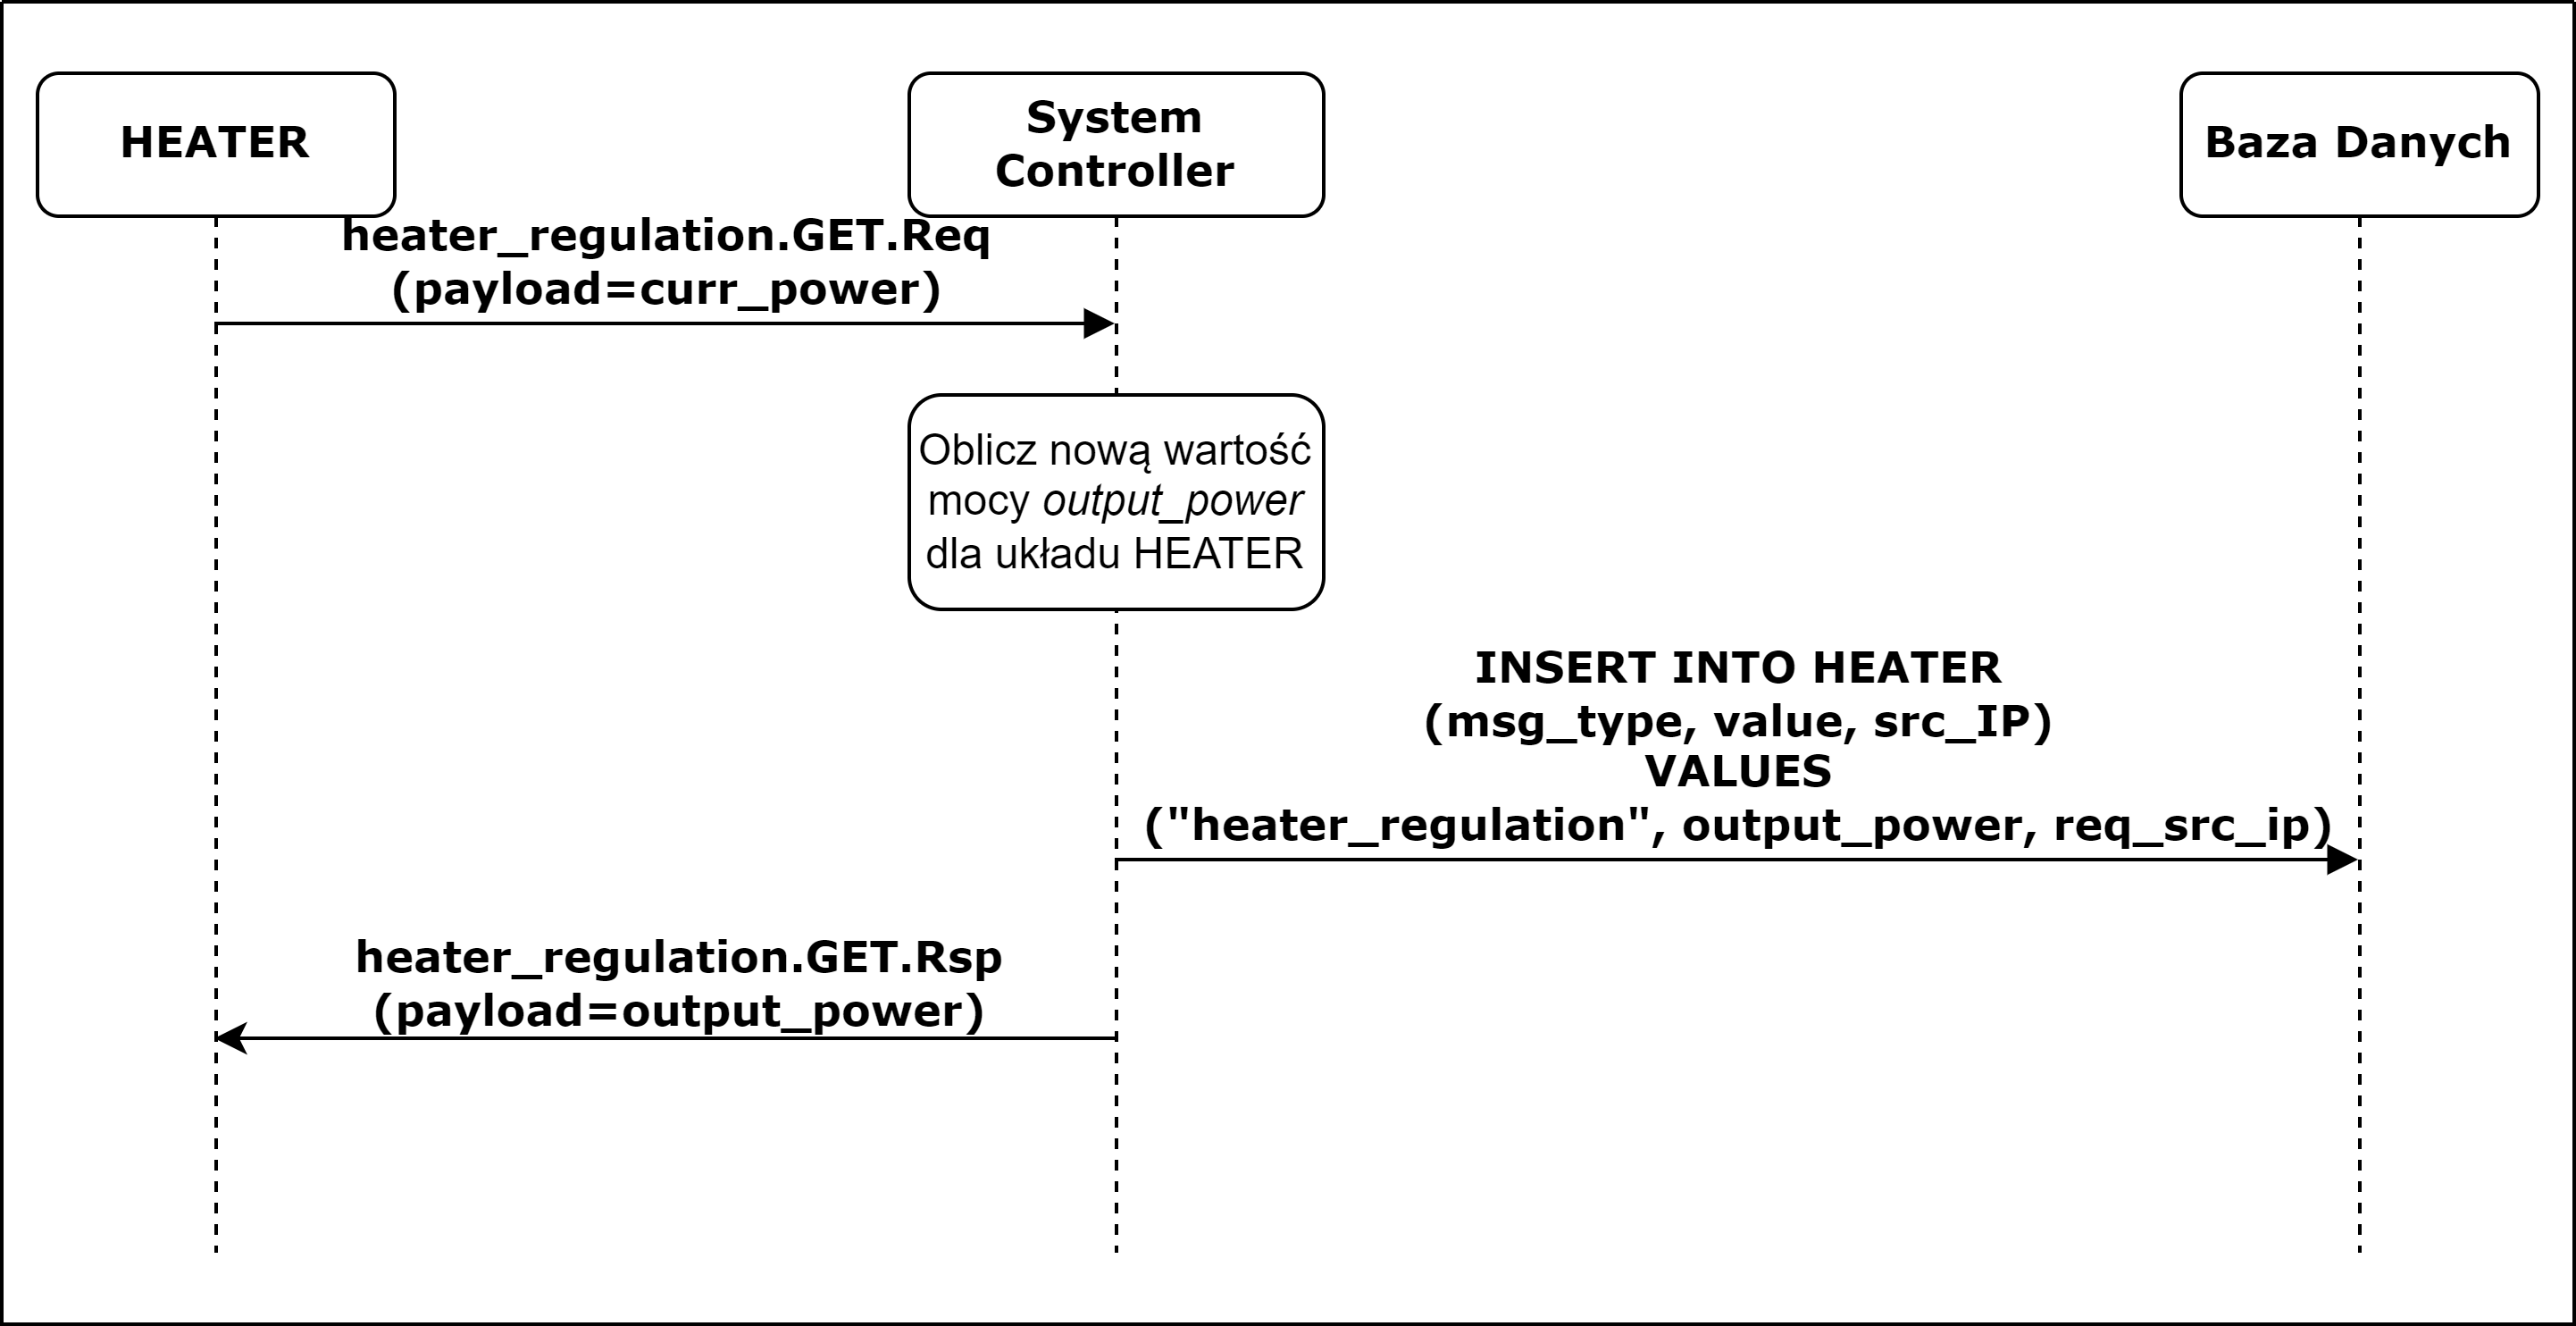
\includegraphics[width=0.8\linewidth]{graphics/sequence-diagrams/heater-regulate-seq.png}
                \caption{Diagram sekwencji regulacji temperatury.}
                \label{fig:seq-heater-regulate}
            \end{figure}

            \begin{figure}[H]
                \centering
                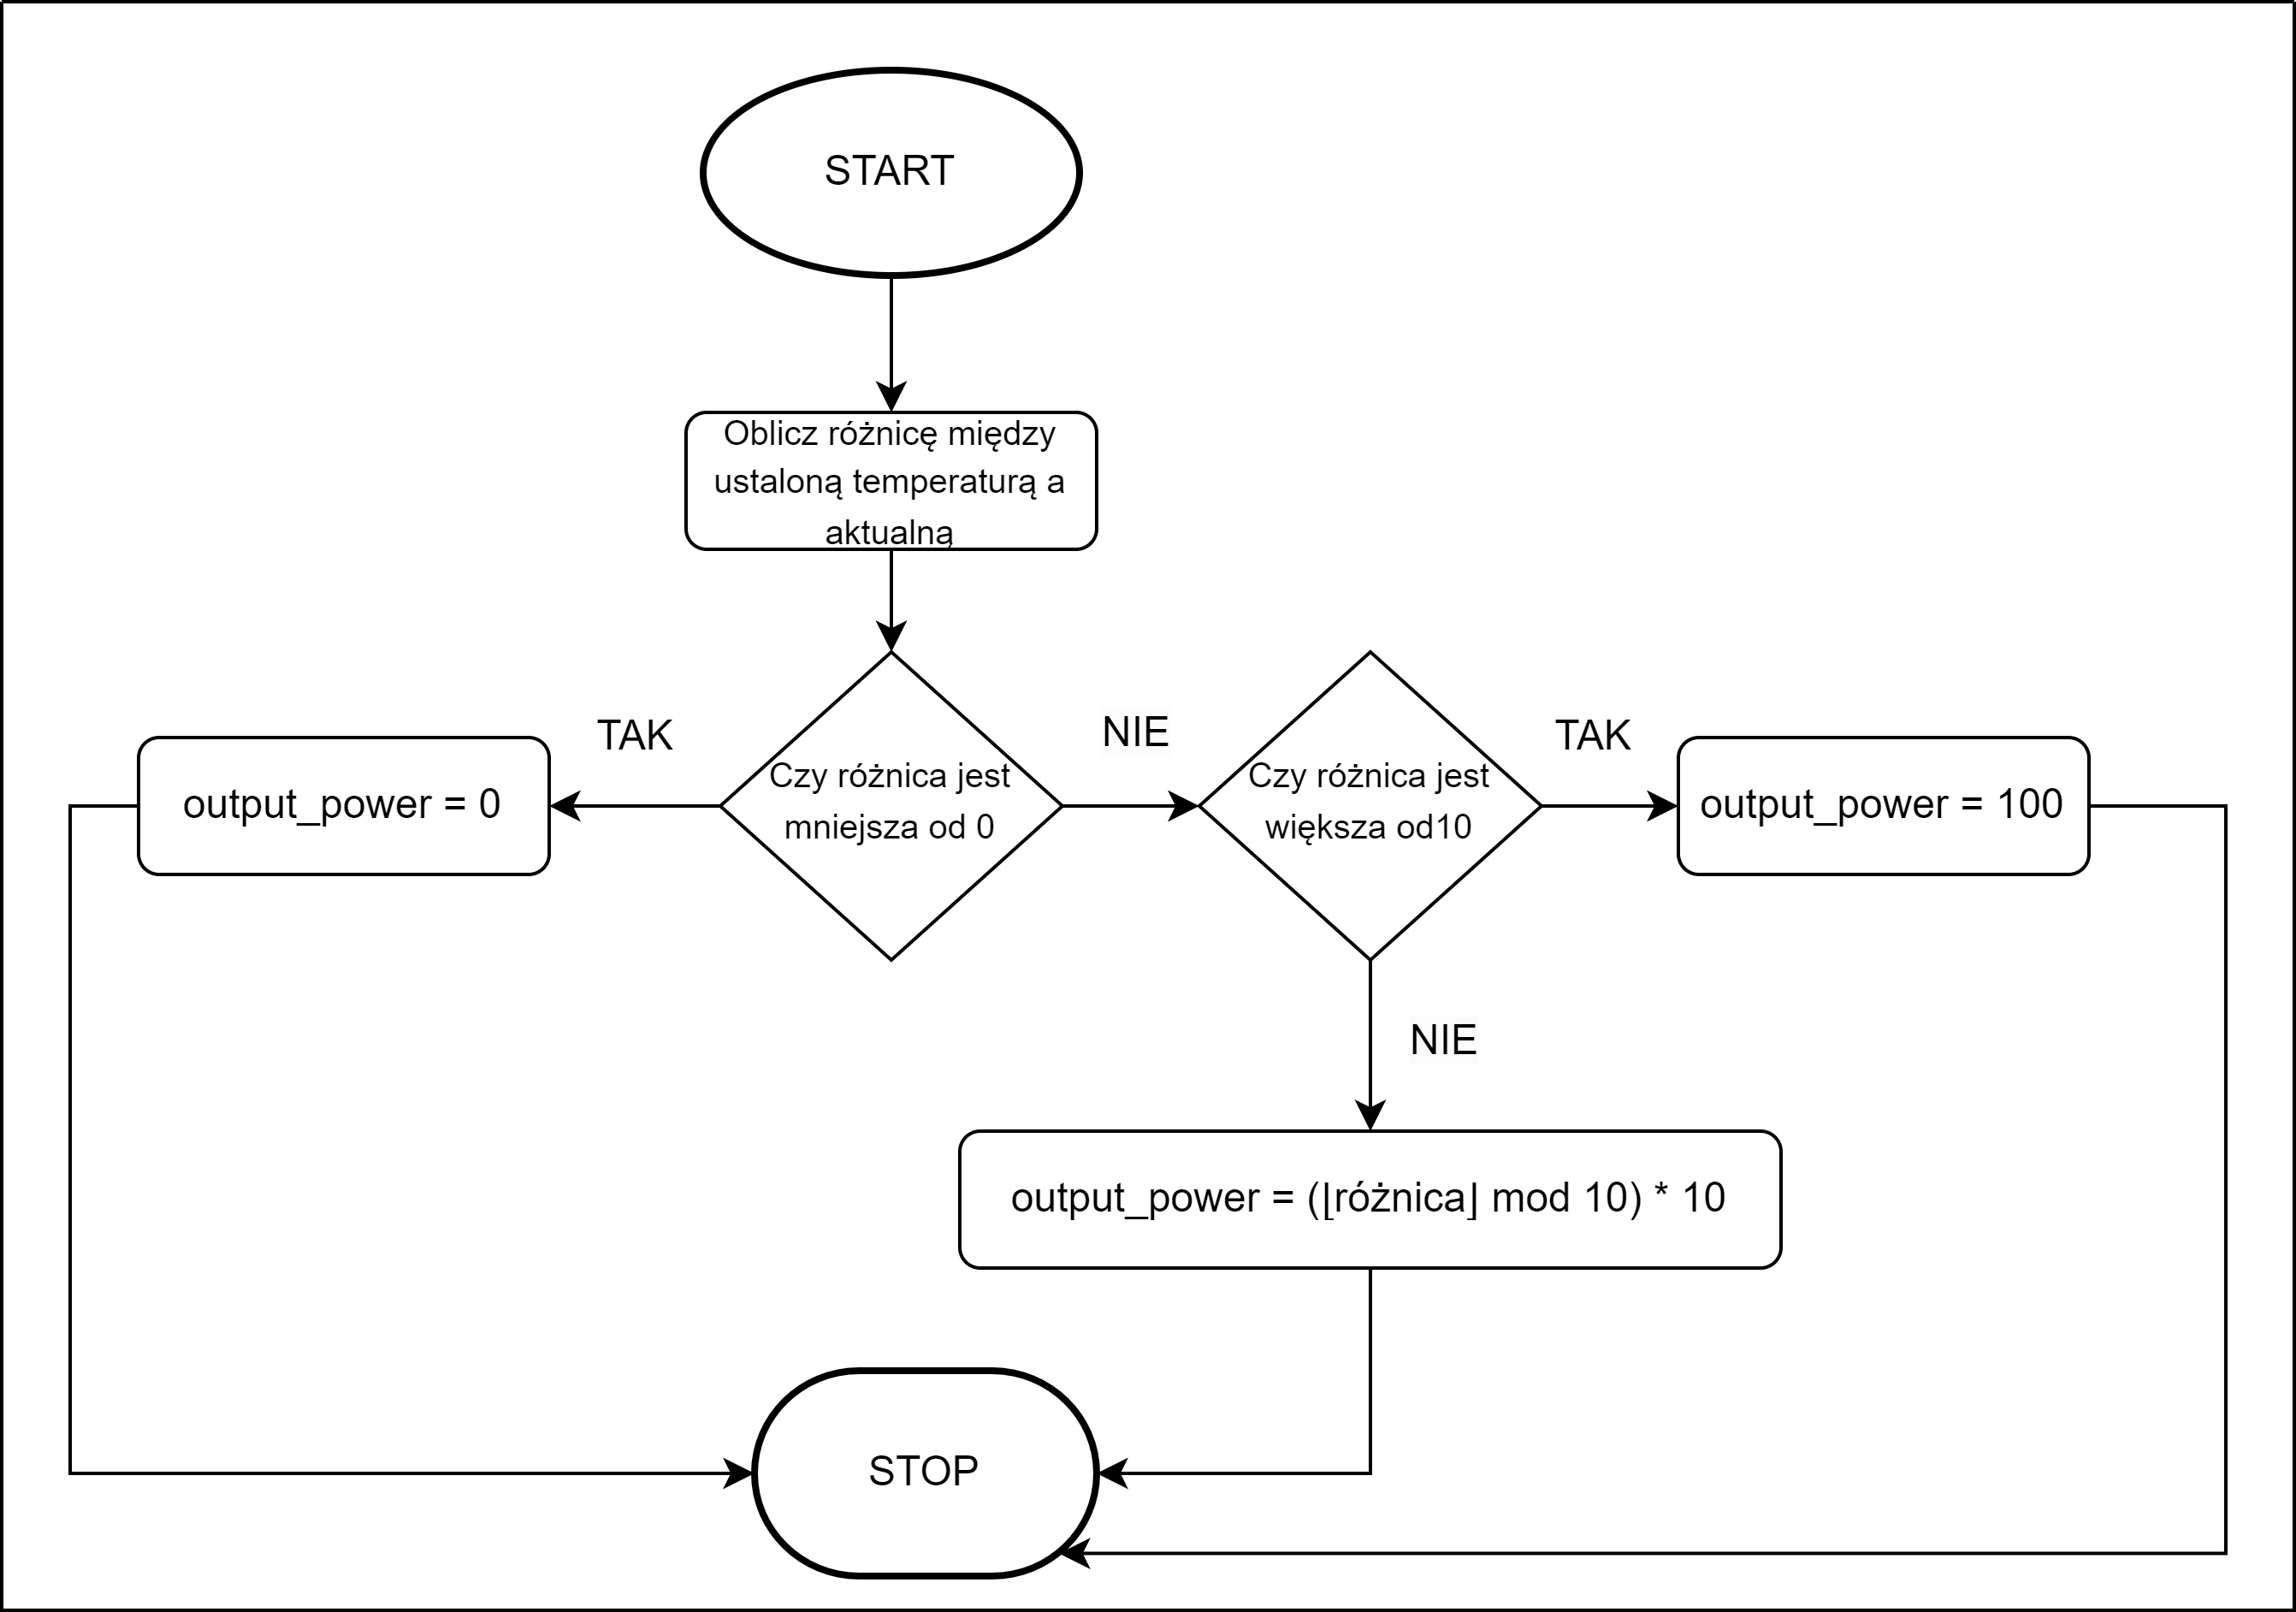
\includegraphics[width=0.8\linewidth]{graphics/heater-block-diagram.png}
                \caption{Algorytm obliczania parametru mocy dla układu HEATER.}
                \label{fig:seq-heater-algo}
            \end{figure}

            Kolejnymi krokami regulacji temperatury w fazie regulacji są:
            \begin{enumerate}
                \item Urządzenie HEATER wysyła zapytanie do System Controllera o otrzymanie nowego parametru regulacji w zasobie \textit{heater\_regulation}, w którym umieszcza aktualną wartość parametru regulacji \textit{curr\_power}.
                \item System Controller oblicza nową wartość \textit{output\_power} na podstawie aktualnej temperatury, umieszczonej w zasobie \textit{temperature} oraz aktualnej wartości parametru regulacji \textit{curr\_power}, zgodnie z algorytmem przedstawionym na Rysunku \ref{fig:seq-heater-algo}.
                \item System Controller loguje informację o przetworzonym zapytaniu, umieszczając obliczoną wartość \textit{output\_power} w tabeli HEATER Bazy Danych.
                \item System Controller odpowiada układowy HEATER, dostarczając nową wartość parametru regulacji \textit{output\_power}.
            \end{enumerate}

            Na Rysunku \ref{fig:seq-dimmer-regulate} zilustrowano przepływ wiadomości między komponentami systemu w fazie regulacji natężenia oświetlenia.

            \begin{figure}[H]
                \centering
                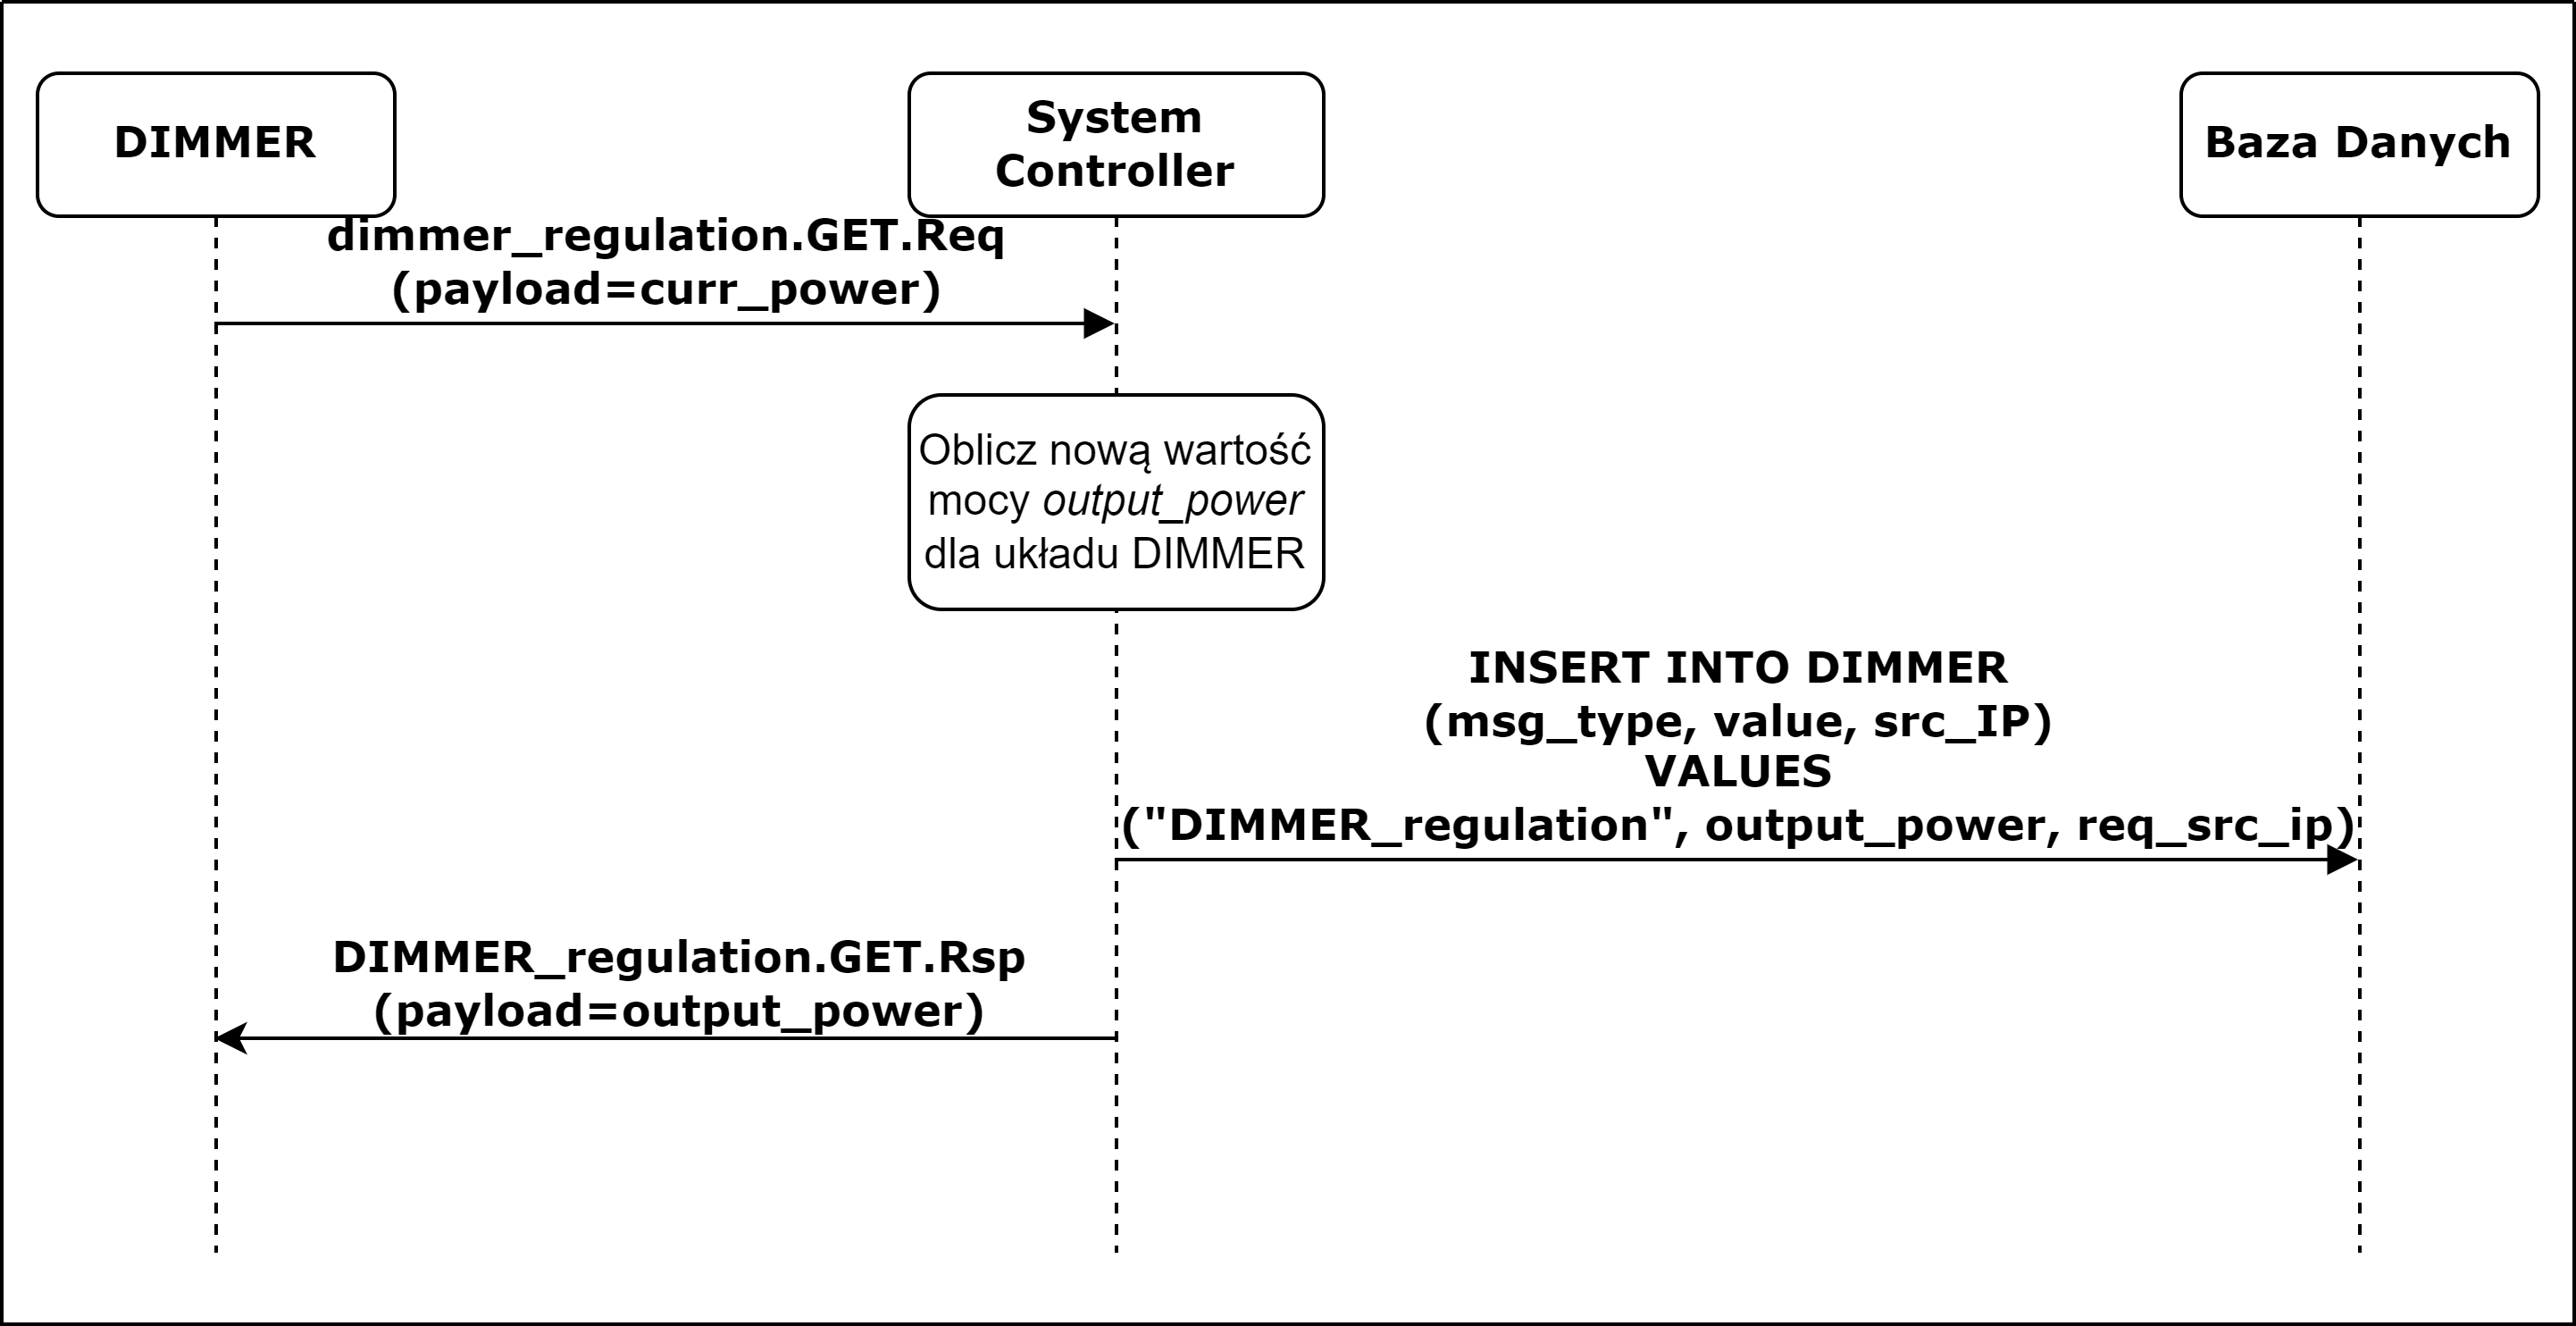
\includegraphics[width=0.8\linewidth]{graphics/sequence-diagrams/dimmer-regulate-seq.png}
                \caption{Diagram sekwencji regulacji natężenia oświetlenia.}
                \label{fig:seq-dimmer-regulate}
            \end{figure}

            \begin{figure}[H]
                \centering
                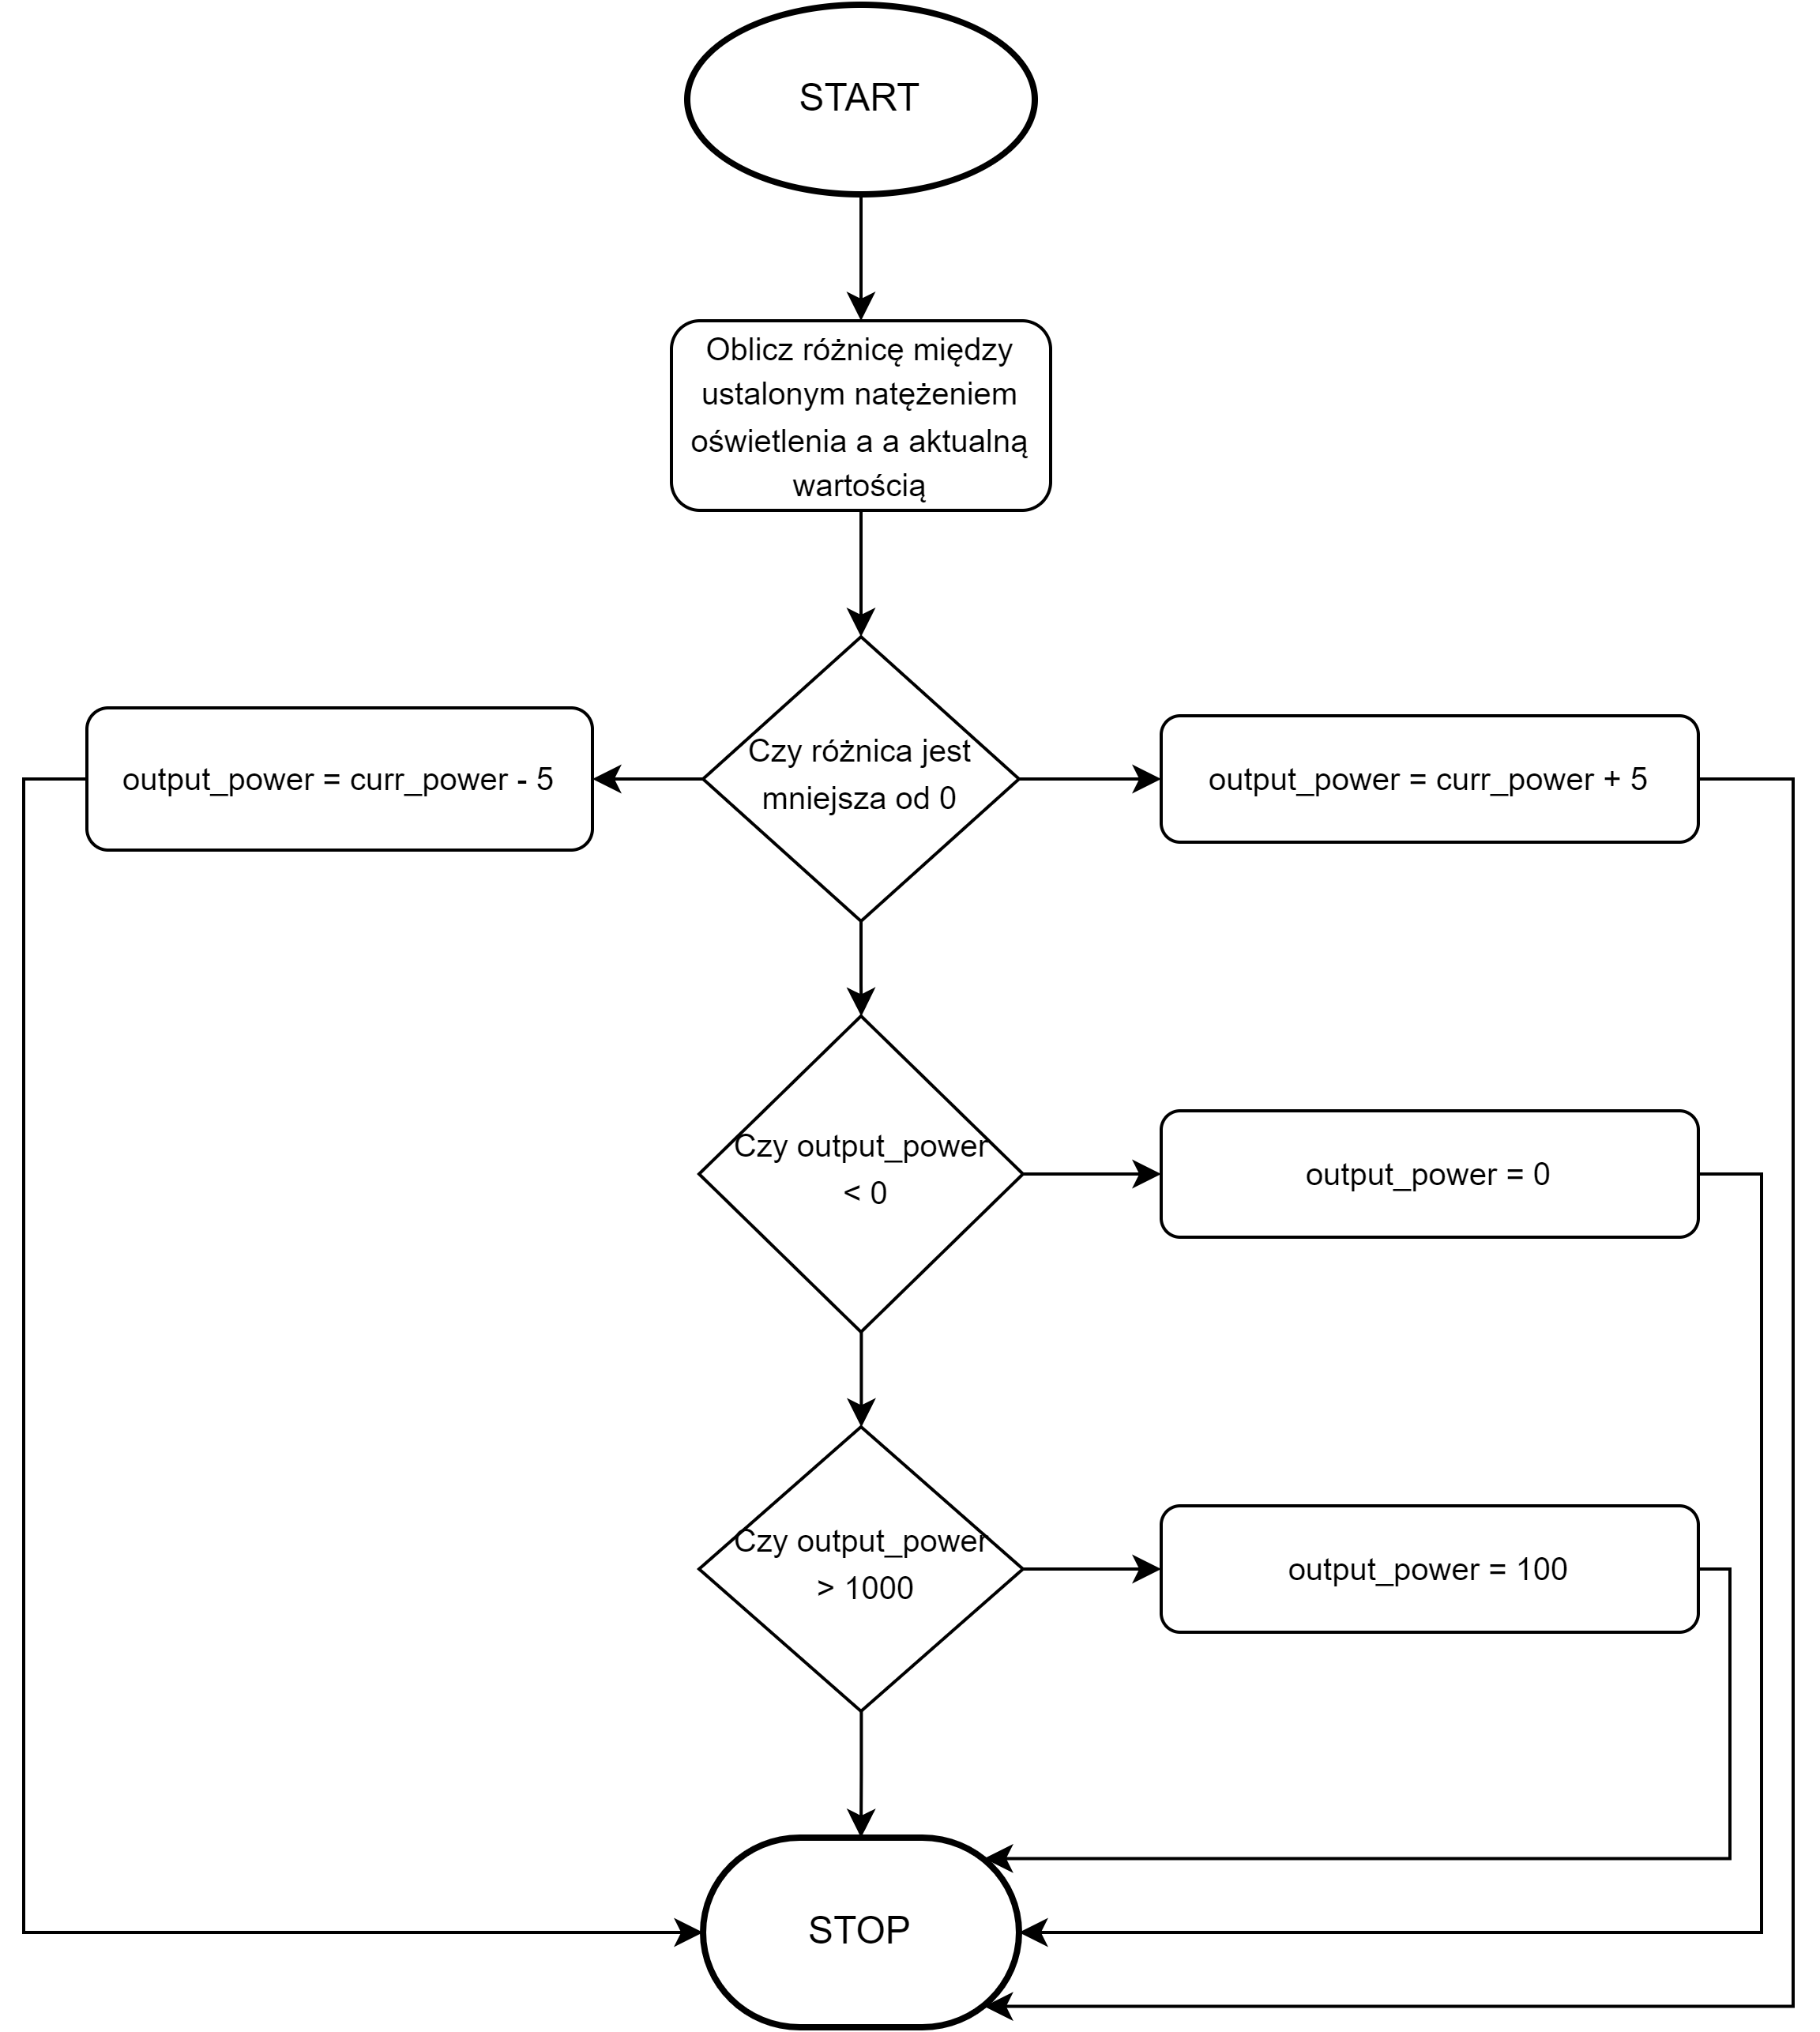
\includegraphics[width=0.8\linewidth]{graphics/dimmer-block-diagram.png}
                \caption{Algorytm obliczania parametru regulacji dla układu DIMMER.}
                \label{fig:seq-dimmer-algo}
            \end{figure}

            Kolejnymi krokami regulacji natężenia oświetlenia w fazie regulacji są:
            \begin{enumerate}
                \item Urządzenie DIMMER wysyła zapytanie do System Controllera o otrzymanie nowego parametru regulacji w zasobie \textit{dimmer\_regulation}, w którym umieszcza aktualną wartość parametru regulacji \textit{curr\_power}.
                \item System Controller oblicza nową wartość \textit{output\_power} na podstawie wartości aktualnego natężenia oświetlenia, umieszczonego w zasobie \textit{illuminance} oraz poprzedniej wartości parametru regulacji \textit{curr\_power}, zgodnie z algorytmem przedstawionym na Rysunku \ref{fig:seq-dimmer-algo}.
                \item System Controller loguje informację o przetworzonym zapytaniu, umieszczając obliczoną wartość \textit{output\_power} w tabeli DIMMER Bazy Danych.
                \item System Controller odpowiada układowy DIMMER, dostarczając nową wartość parametru regulacji \textit{output\_power}.
            \end{enumerate}

            W związku z charakterem pracy, w której nacisk implementacji projektu został położony na aspekty komunikacji, dobrane algorytmy przedstawione na Rysunku \ref{fig:seq-heater-algo} oraz Rysunku \ref{fig:seq-dimmer-algo} pozwalają na zaprezentowanie działania prototypowego systemu, natomiast nie są optymalne. We wdrożonych algorytmach System Controllera brakuje histerezy, co w konsekwencji mogłoby spowodować skokowe zmiany obliczanego parametru regulacji przy niewielkich odchyleniach wartości temperatury oraz natężenie oświetlenia środowiska w stosunku do zadanego stanu. Opisane zachowanie mogłoby mieć wpływ na żywotność baterii urządzeń, które pracują jako regulator. Jednym z rozwiązań problemu mogłoby być zastosowanie w System Controllerze algorytmu opartego o PID (ang. \textit{Proportional-Integral-Derivative}).
